% ============================================================
% Market Power and the Gender Career Gap
% Short proposal for faculty circulation
% ============================================================
\documentclass[11pt]{article}

% ---------- packages ----------
\usepackage[english]{babel}
\usepackage{johd}
\usepackage{amsmath, mathtools, mathrsfs}
\usepackage{bm, amssymb, bbm}
\usepackage{xcolor}
\usepackage{subcaption}

\hypersetup{colorlinks=true, linkcolor=blue, citecolor=blue, urlcolor=blue}

% ---------- tighter spacing for short proposal ----------
%\linespread{1.08}
%\setlength{\parskip}{3pt}

% ============================================================
\title{Market Power and Gender Gaps in Career Dynamics: \\ Evidence from Matched HR Records in Chile}
\author{Sofia Valdivia \\ Duke University}
\date{\today}

\begin{document}
\maketitle

% ============================================================
% 1. INTRODUCTION AND LITERATURE
% ============================================================

% ============ V2: REWRITTEN INTRO (JNS style) ============
\section{Introduction and Related Literature}

Gender gaps in wages and career outcomes have narrowed over recent decades but remain substantial, even as women have surpassed men in educational attainment and fertility rates have declined. A large literature documents remaining wage differences and connects them to human capital, occupational sorting, the motherhood penalty, and statistical discrimination \citep{goldin_grand_2014, blau_gender_2017, kleven_children_2019, Xiao}. But wages are only one dimension of how careers develop. Firms also decide who gets hired and who gets promoted, and these decisions shape career trajectories in ways that wage analysis alone cannot capture. This paper asks whether labor market power distorts these firm-side decisions differently for men and women.

\paragraph{Imperfect competition in labor markets.}
Search frictions give firms market power over their workers, allowing wages to fall below marginal product \citep{manning_monopsony_2003, manning_imperfect_2011}. A class of on-the-job search models shows how this power operates: firms set wages to balance profit margins against the risk of losing workers to competitors, and workers' outside options determine their bargaining position \citep{burdett_wage_1998, postel-vinay_equilibrium_2002}. Empirically, labor supply elasticities to individual firms are low \citep{sokolova_monopsony_2021}, and both the structure of local labor markets and the degree of job differentiation generate substantial welfare losses \citep{berger_labor_2022, Jarosch_Nimczik_Sorkin_2024}. This paper builds on the insight that outside options shape the employment relationship, but extends it from wages to career dynamics.

\paragraph{Outside options and gender.}
A growing literature shows that women face fewer outside options than men in the labor market, and that this gap depresses their wages. Women exhibit lower labor supply elasticities to individual firms \citep{webber_firm-level_2016, sharma_monopsony_2023}, and differences in outside options, driven in part by commuting costs and geographic mobility, explain a meaningful share of the gender wage gap \citep{caldwell_outside_nodate, morchio_gender_2024, caldwell_gender_2022}. On the firm side, women capture a smaller share of firm-specific pay premiums \citep{card_bargaining_2016}. This literature establishes that imperfect competition matters for gender wage gaps, but it has focused exclusively on wages. I extend the analysis to hiring and promotion decisions.

\paragraph{Gender and career dynamics.}
A separate literature documents gender gaps in hiring and promotion but has not connected them to market structure. Subjective assessments of worker ``potential'' account for roughly half of the gender promotion gap \citep{benson_potential_2026}, and employers screen applicants differently by gender, with discrimination concentrated among specific firms \citep{bertrand_are_2004, kline_systemic_2022}. These studies provide rich within-firm evidence but do not ask how the competitive environment shapes these decisions. %This paper fills that gap.

\paragraph{This paper.}
I connect imperfect competition in labor markets to gender gaps in career dynamics. The mechanism is that if women face lower outside offer arrival rates than men, firms have less competitive pressure to promote them. A firm deciding whether to promote a junior employee weighs the output gain against the wage increase, but also considers retention: promoting raises the worker's continuation value, reducing the probability she leaves. When a male worker has many outside options, the firm promotes to retain him. When a female worker has fewer options, a firm can delay the promotion at little cost. The result is a higher promotion bar for women, driven not by productivity differences but by the competitive structure of the labor market. At the hiring margin, the prediction is ambiguous: women who are hired stay longer (favoring lower screening thresholds), but women with fewer alternatives continue to apply even when the bar is high (favoring higher thresholds). Which force dominates is an empirical question.

I (will) develop an on-the-job search model building on \citet{burdett_wage_1998} and \citet{postel-vinay_equilibrium_2002}, extended with an internal promotion decision following \citet{gibbons_theory_1999} and gender-specific outside options following \citet{sharma_monopsony_2023}. The empirical analysis uses administrative data from BUK, an HR platform covering over 19,000 Chilean firms and 4.7 million workers, including a recruitment module with 186,000 selection processes. Chile provides policy variation; three overlapping reforms during the sample period shift different parameters of the firm's problem, offering scope for identification. The contribution is to connect monopsony to career dynamics at both the hiring and promotion margins, using matched employer-employee-applicant data to observe how firms with different degrees of market power make these decisions for men and women.

% ============ V1: ORIGINAL INTRO (preserved) ============
\iffalse
% --- Original Section 1 (commented out) ---

Gender gaps in the labor market have persisted despite decades of convergence in education and declining fertility. A large literature documents wage differences between men and women and connects them to human capital, occupational sorting, and the motherhood penalty \citep{goldin_grand_2014, blau_gender_2017, kleven_children_2019}. But wages are only one dimension of how careers develop. Firms also decide who gets hired and who gets promoted, and these decisions shape career trajectories in ways that wage analysis alone cannot capture. This paper proposes to study whether labor market power distorts these firm-side decisions differently for men and women.

A growing body of work shows that monopsony power depresses women's wages more than men's. \citet{webber_firm-level_2016} finds that women face greater search frictions, with the resulting monopsony wedge explaining a meaningful share of the gender wage gap. \citet{sharma_monopsony_2023} estimates that market power accounts for a significant portion of the gender pay gap. \citet{caldwell_outside_nodate} show that differences in outside options explain 20 percent of the gender wage gap in Germany. On the firm side, \citet{card_bargaining_2016} find that women capture only 90 percent of firm-specific pay premiums in Portugal. This literature establishes that market power matters for gender wage gaps, but it has focused exclusively on wages. A separate literature documents gender gaps in career dynamics---\citet{benson_potential_2026} show that subjective ``potential'' assessments account for half of the promotion gap; \citet{bertrand_are_2004} and \citet{kline_systemic_2022} document differential screening by gender at hiring---but does not connect these patterns to market structure.

I propose to connect these literatures. If women face fewer outside options than men, firms have less competitive pressure to hire them fairly or to promote them quickly. Consider a firm deciding whether to promote a junior employee. Beyond the output gain and wage increase, there is a retention motive: promoting raises the worker's continuation value, making outside offers less attractive. When a male worker has many outside options, the firm promotes to retain him. When a female worker has fewer options, the retention motive is weaker---the firm can delay at little cost. The result is a higher promotion bar for women, driven not by productivity differences but by the competitive structure of the labor market. At the hiring margin, the prediction is ambiguous: women who are hired stay longer (favoring lower screening thresholds), but women with fewer alternatives continue to apply even when the bar is high (favoring higher thresholds). Which force dominates is an empirical question.

The model builds on \citet{burdett_wage_1998}, extended with promotions following \citet{gibbons_theory_1999}, gender-specific outside options from \citet{sharma_monopsony_2023}, and the retention logic of \citet{postel-vinay_equilibrium_2002}. The empirical analysis uses administrative data from BUK, an HR platform covering over 19,000 Chilean firms and 4.7 million workers, including a recruitment module with 186,000 selection processes. Chile provides policy variation---three overlapping reforms during the sample period shift different parameters of the firm's problem---offering scope for identification. The contribution is to connect monopsony to career dynamics at both the hiring and promotion margins, using matched employer-employee-applicant data to observe how firms with different degrees of market power make these decisions for men and women.

\fi
% ============ END V1 ============
% ============================================================
% 2. SETTING
% ============================================================
\section{Setting}

Chile provides a natural setting for studying gender gaps and market power. Women have surpassed men in educational attainment\footnote{The tertiary education attainment rate is 45\% for women versus 37\% for men \citep{oecd_education_2024}.} and the total fertility rate has fallen to 1.03, one of the lowest in the region \citep{ine_anuario_2024}. Yet the gender wage gap persists at 15 to 20 percent and female labor force participation remains at roughly 53\%, well below the OECD average of 65\%. These gaps, combined with rising informality, have become a central topic of public debate and prompted a series of labor market reforms during the 2022--2026 period that this paper exploits for identification.

Three reforms are particularly relevant. First, a reduction in the standard workweek from 45 to 40 hours (Ley 21.561), phased in three steps between April 2024 and April 2028, which changes the premium on long-hours availability. Second, a flexible work law for workers with caregiving responsibilities (Ley 21.645), effective January 2024, which grants parents of children under 14 the right to request flexible or remote work, possibly expanding outside options for women as primary caregivers. Third, the childcare mandate under Article 203 of the Labor Code, which requires firms employing 20 or more women to provide or fund childcare, creating a discontinuity in the cost of employing women at a known firm-size threshold. Each reform shifts a different parameter of the firm's problem and can be exploited for identification.

% ============================================================
% 3. DATA
% ============================================================
\section{Data}

\subsection{Platform and data structure}

The empirical analysis draws on administrative records from BUK, an HR and payroll platform used by Chilean firms across all 20 ISIC sectors. BUK records each stage of the employment relationship: (i) \textbf{hiring}, through a recruitment module that tracks vacancies, applications, candidate demographics, referral sources, and application scores; (ii) \textbf{employment contracts}, with dates, job titles, areas, contract types, workday types, and supervisor identifiers; (iii) \textbf{monthly payroll}, including base, gross, net salary, and monetary bonuses based on performance or tenure ; (iv) \textbf{promotions}, identified through changes in role and accompanying salary increases; and (v) \textbf{separations}, with spell end dates observed for 83.2\% of completed spells. The panel covers 2022 to 2026. Table~\ref{tab:summary} summarizes the sample.

\begin{table}[h]
\centering
\caption{Sample summary (Chile, 2022--2026)}
\label{tab:summary}
\begin{tabular}{lr}
\hline
Firms                        & 19,338 \\
Unique workers               & 4,712,667 \\
Job spells                   & 8,273,604 \\
Male / Female                & 62.8\% / 37.2\% \\
\hline
Selection processes          & 186,457 \\
Applications                 & 2,725,982 \\
Unique candidates            & 839,664 \\
Candidate gender: Male / Female & 56.0\% / 43.0\% \\
\hline
\end{tabular}
\end{table}

Supervisor identifiers enable measurement of organizational hierarchy and promotion events, while the recruitment module allows direct observation of the hiring pipeline from application through scoring.

\subsection{Sample selection}

BUK is not a random sample of Chilean firms. Adoption is voluntary, and the platform is marketed primarily to mid-to-large employers. Table~\ref{tab:selection} compares the BUK sample to the SII (Servicio de Impuestos Internos) universe of formal Chilean firms.

\begin{table}[h]
\centering
\caption{BUK vs.\ SII universe: firm size (2023)}
\label{tab:selection}
\begin{tabular}{lrrrr}
\hline
 & \multicolumn{2}{c}{Firms (\%)} & \multicolumn{2}{c}{Workers (\%)} \\
Size & BUK & SII & BUK & SII \\
\hline
Micro/Small  & 39.6 & 95.3 & 5.7  & 29.9 \\
Medium       & 31.9 &  3.2 & 14.5 & 16.5 \\
Large        & 28.5 &  1.5 & 79.8 & 53.6 \\
\hline
\end{tabular}
\end{table}

Micro and small firms are under-represented relative to the SII universe, while large firms are over-represented. In terms of sector composition, public administration is structurally absent (public-sector employers do not use the platform). Wholesale \& retail, transport, and construction is under-represented, while real estate, professional \& tech, and finance \& insurance are over-represented. %Wholesale and retail trade and construction are roughly in line with the economy-wide distribution.

The over-representation of large firms is an advantage in that the model's predictions are most relevant for firms with structured hiring pipelines and internal promotion ladders. The main limitation is that the sample does not capture thin local labor markets where small employers dominate.

% ============================================================
% 4. REDUCED FORM EVIDENCE
% ============================================================
\section{Preliminary Evidence}

This section presents \textbf{preliminary} descriptive evidence motivating the structural model. I organize the evidence around three questions: how much does employer market power vary across labor markets, do gender gaps in career outcomes vary with market power, and do workers' own perceptions support the patterns in the administrative data? %Several important pieces of evidence, including job-to-job transition rates and application-to-hire conversion rates, are still in progress. I discuss these at the end of the section.


\paragraph{Measuring market concentration.} I measure labor market concentration using the Herfindahl Hirschman Index (HHI) following \citet{azar_labor_2022}.\footnote{\citet{sharma_monopsony_2023} shows that HHI underdiagnoses gender differences in concentration because it does not account for women's disproportionate employment in fewer occupations. In future work, I plan to complement HHI with structural estimates that distinguish vertical and horizontal sources of monopsony power \citep{sharma_monopsony_2023} and with commuting-based market definitions \citep{Schubert_Stansbury_Taska_2024}.} 
For each market cell $i$, defined as an occupation $\times$ region pair,
\begin{equation*}
    \text{HHI}_{i,t} = \sum_{j = 1}^J s_{j,i,t}^{2}
\end{equation*}
where $s_{j,i} = N_{j} / N_{i}$ is firm $j$'s share of employment in market $i$. I compute two variants: an employment-based measure using year-end headcounts across 8 functional areas and 16 regions (1,017 cells), and a vacancy-based measure using vacancy counts from the recruitment module (618 cells). For the HHI based on vacancies, the market share of a firm is defined as the sum of the vacancies posted by firm $j$ in a given market divided by total vacancies posted in that market.
Figure~\ref{fig:hhi} shows the distribution of both measures. The employment mean HHI is 2,249 (moderately concentrated), but there is a substantial right tail, with pronounced geographic variation from Santiago (HHI of 209) to peripheral regions such as Ays\'en (HHI of 5,690). The vacancy-based measure shows even higher concentration: the mean is 6,073 and 28.5\% of cells are served by a single firm. This is mainly driven by small/remote regions where BUK has only a few firms\footnote{When we apply vacancy-weights, monopoly drops from 28.5\% of cells to just 1.1\%. The unweighted distribution overstates concentration.}.
\begin{figure}[h]
\centering
\begin{subfigure}[t]{0.48\textwidth}
    \centering
    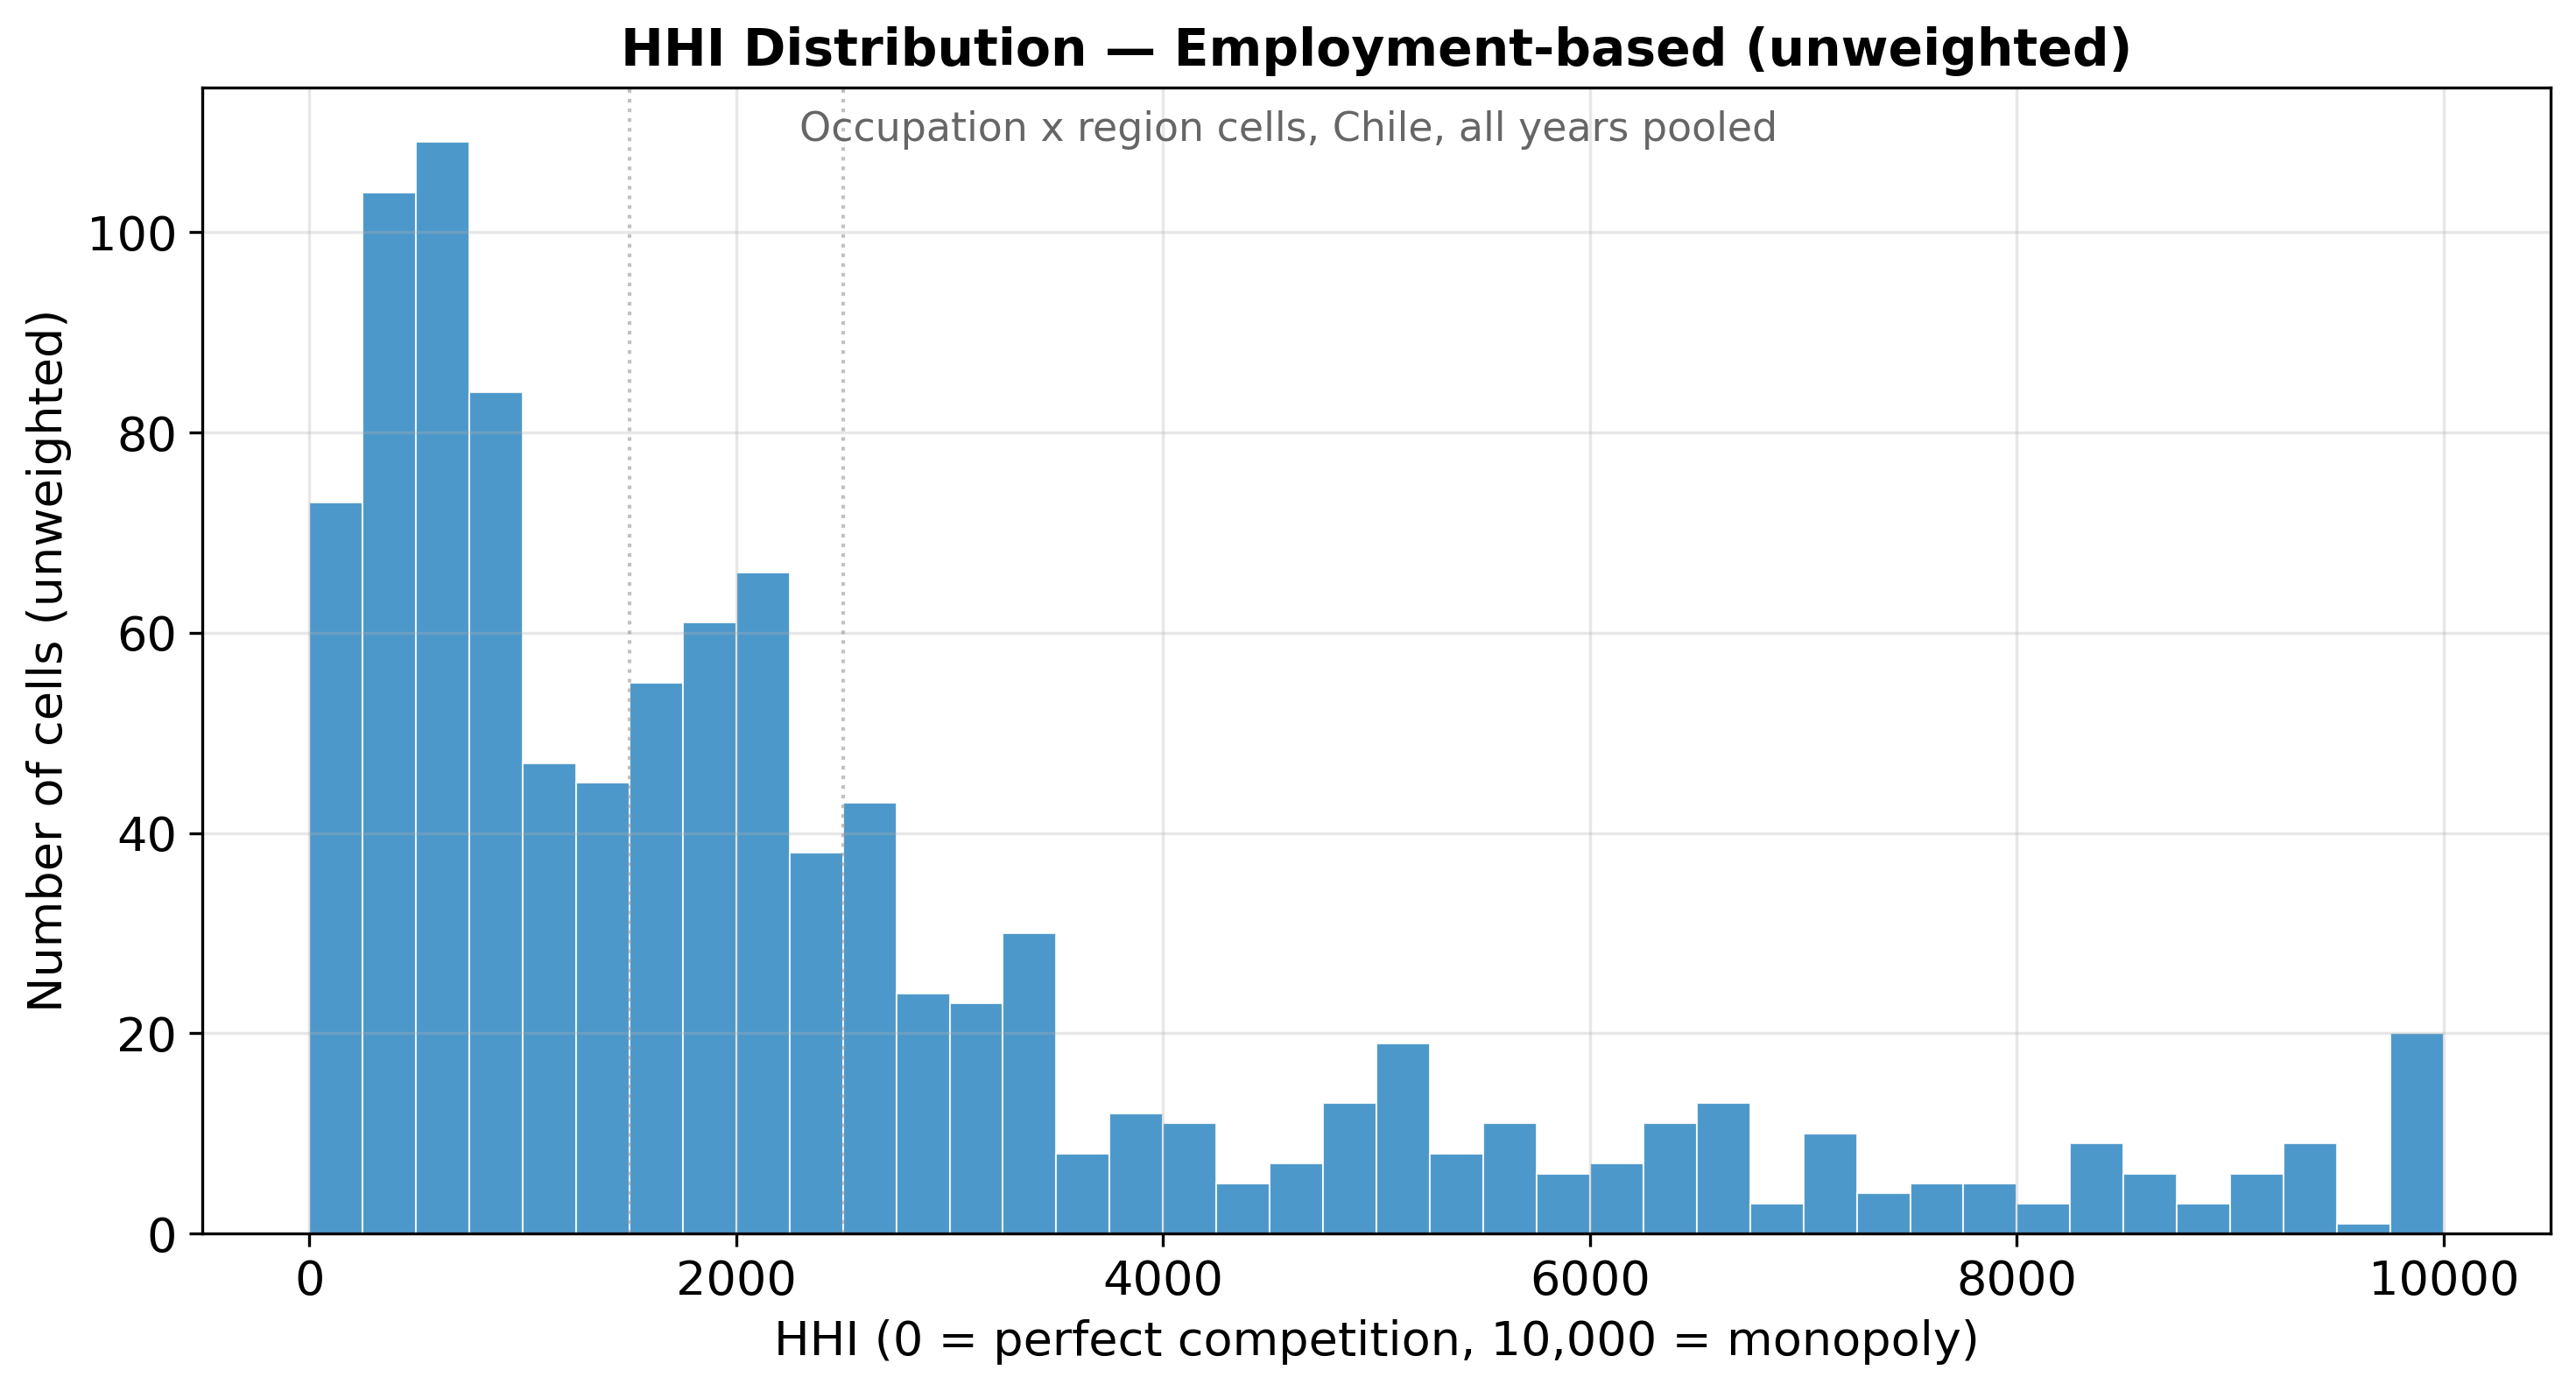
\includegraphics[width=\textwidth]{../../../1_Code/figures/rf_2_4_hhi_distribution_employment_unweighted.png}
    \caption{Employment-based (1,017 cells)}
    \label{fig:hhi_emp}
\end{subfigure}
\hfill
\begin{subfigure}[t]{0.48\textwidth}
    \centering
    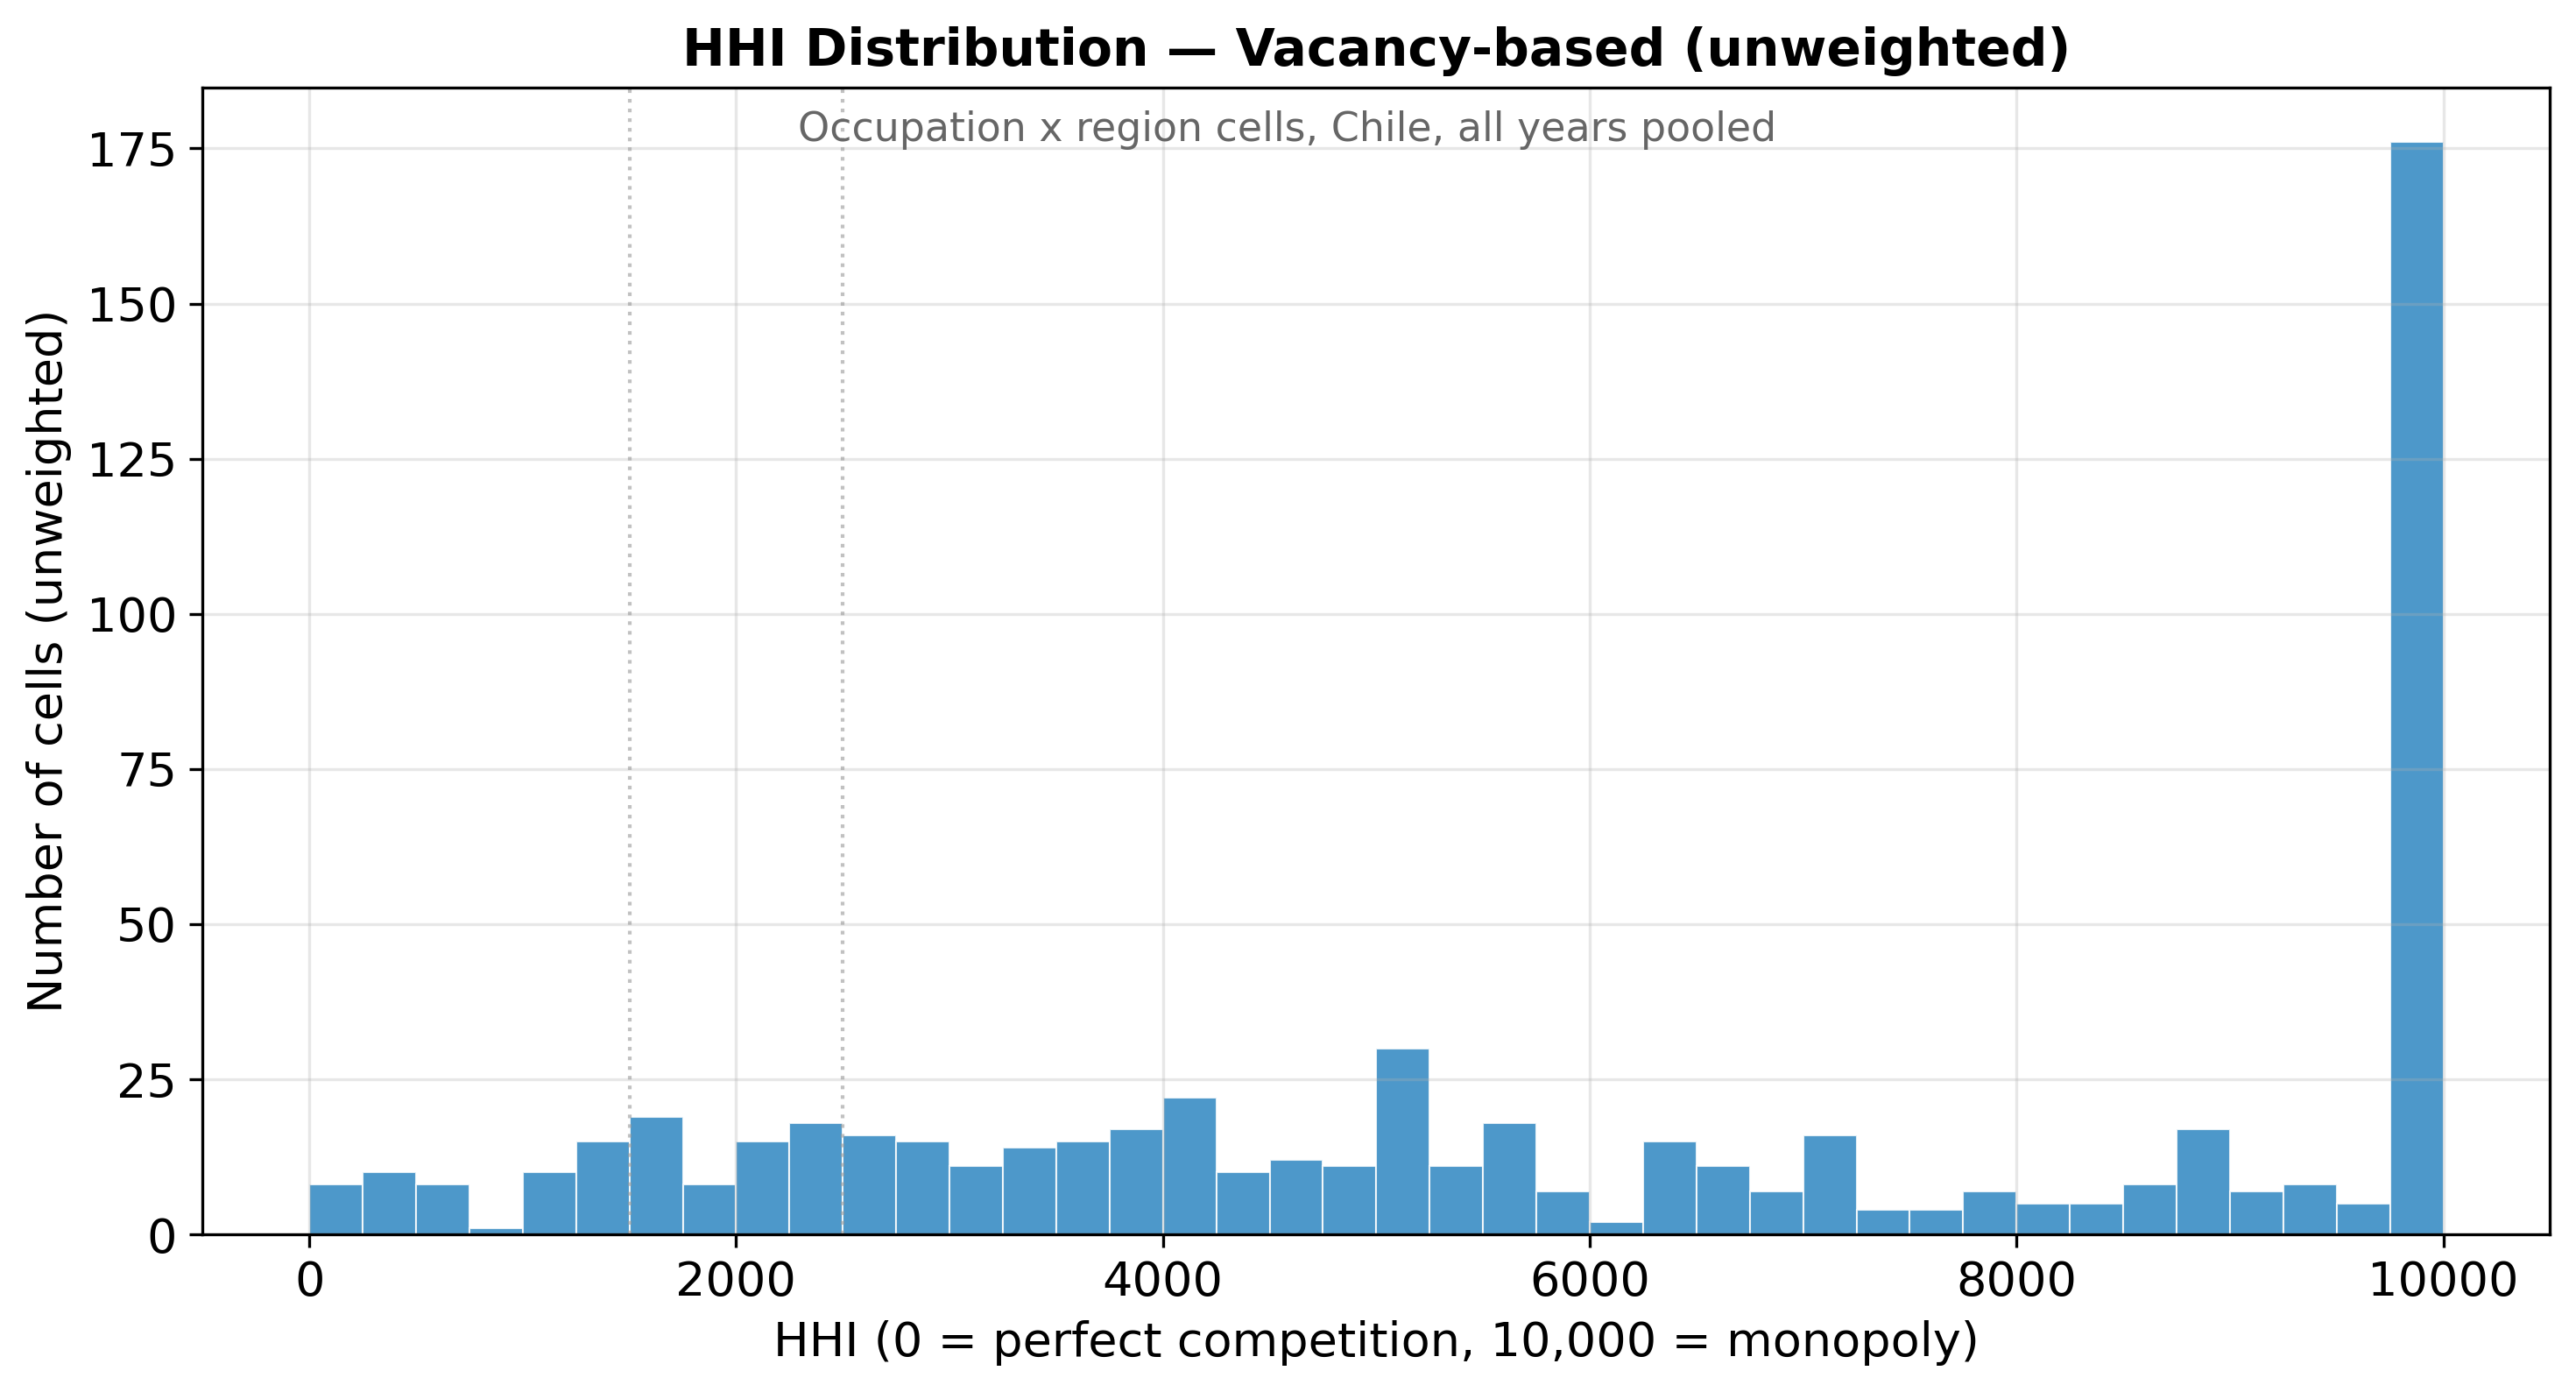
\includegraphics[width=\textwidth]{../../../1_Code/figures/rf_2_4_hhi_distribution_vacancy_unweighted.png}
    \caption{Vacancy-based (618 cells)}
    \label{fig:hhi_vac}
\end{subfigure}
\caption{Distribution of HHI across occupation $\times$ region cells (Chile, all years pooled).}
\label{fig:hhi}
\end{figure}

\paragraph{Promotion gaps and market concentration.} In the current definition of promotion, there is virtually no gender gap in promotion rates: women are promoted at 2.10\% per year and men at 2.04\%, based on 73,000 promotions over 3.5 million person-years. Median entry wages, by contrast, show an 11\% raw gap (CLP 460,000 for women vs.\ 518,000 for men), though this does not condition on occupation or firm.

However, this aggregate similarity hides heterogeneity by market structure. Figure~\ref{fig:promo_hhi} shows that the gender promotion gap reverses with market concentration: in competitive markets women are promoted at higher rates than men, while in concentrated markets men are promoted more. The same pattern appears when splitting by firm size. This reversal is consistent with the retention mechanism in the model: in concentrated markets, where women's outside options are weakest, firms can delay their promotions at little cost. These patterns are descriptive and do not establish causality.

\begin{figure}[h]
\centering
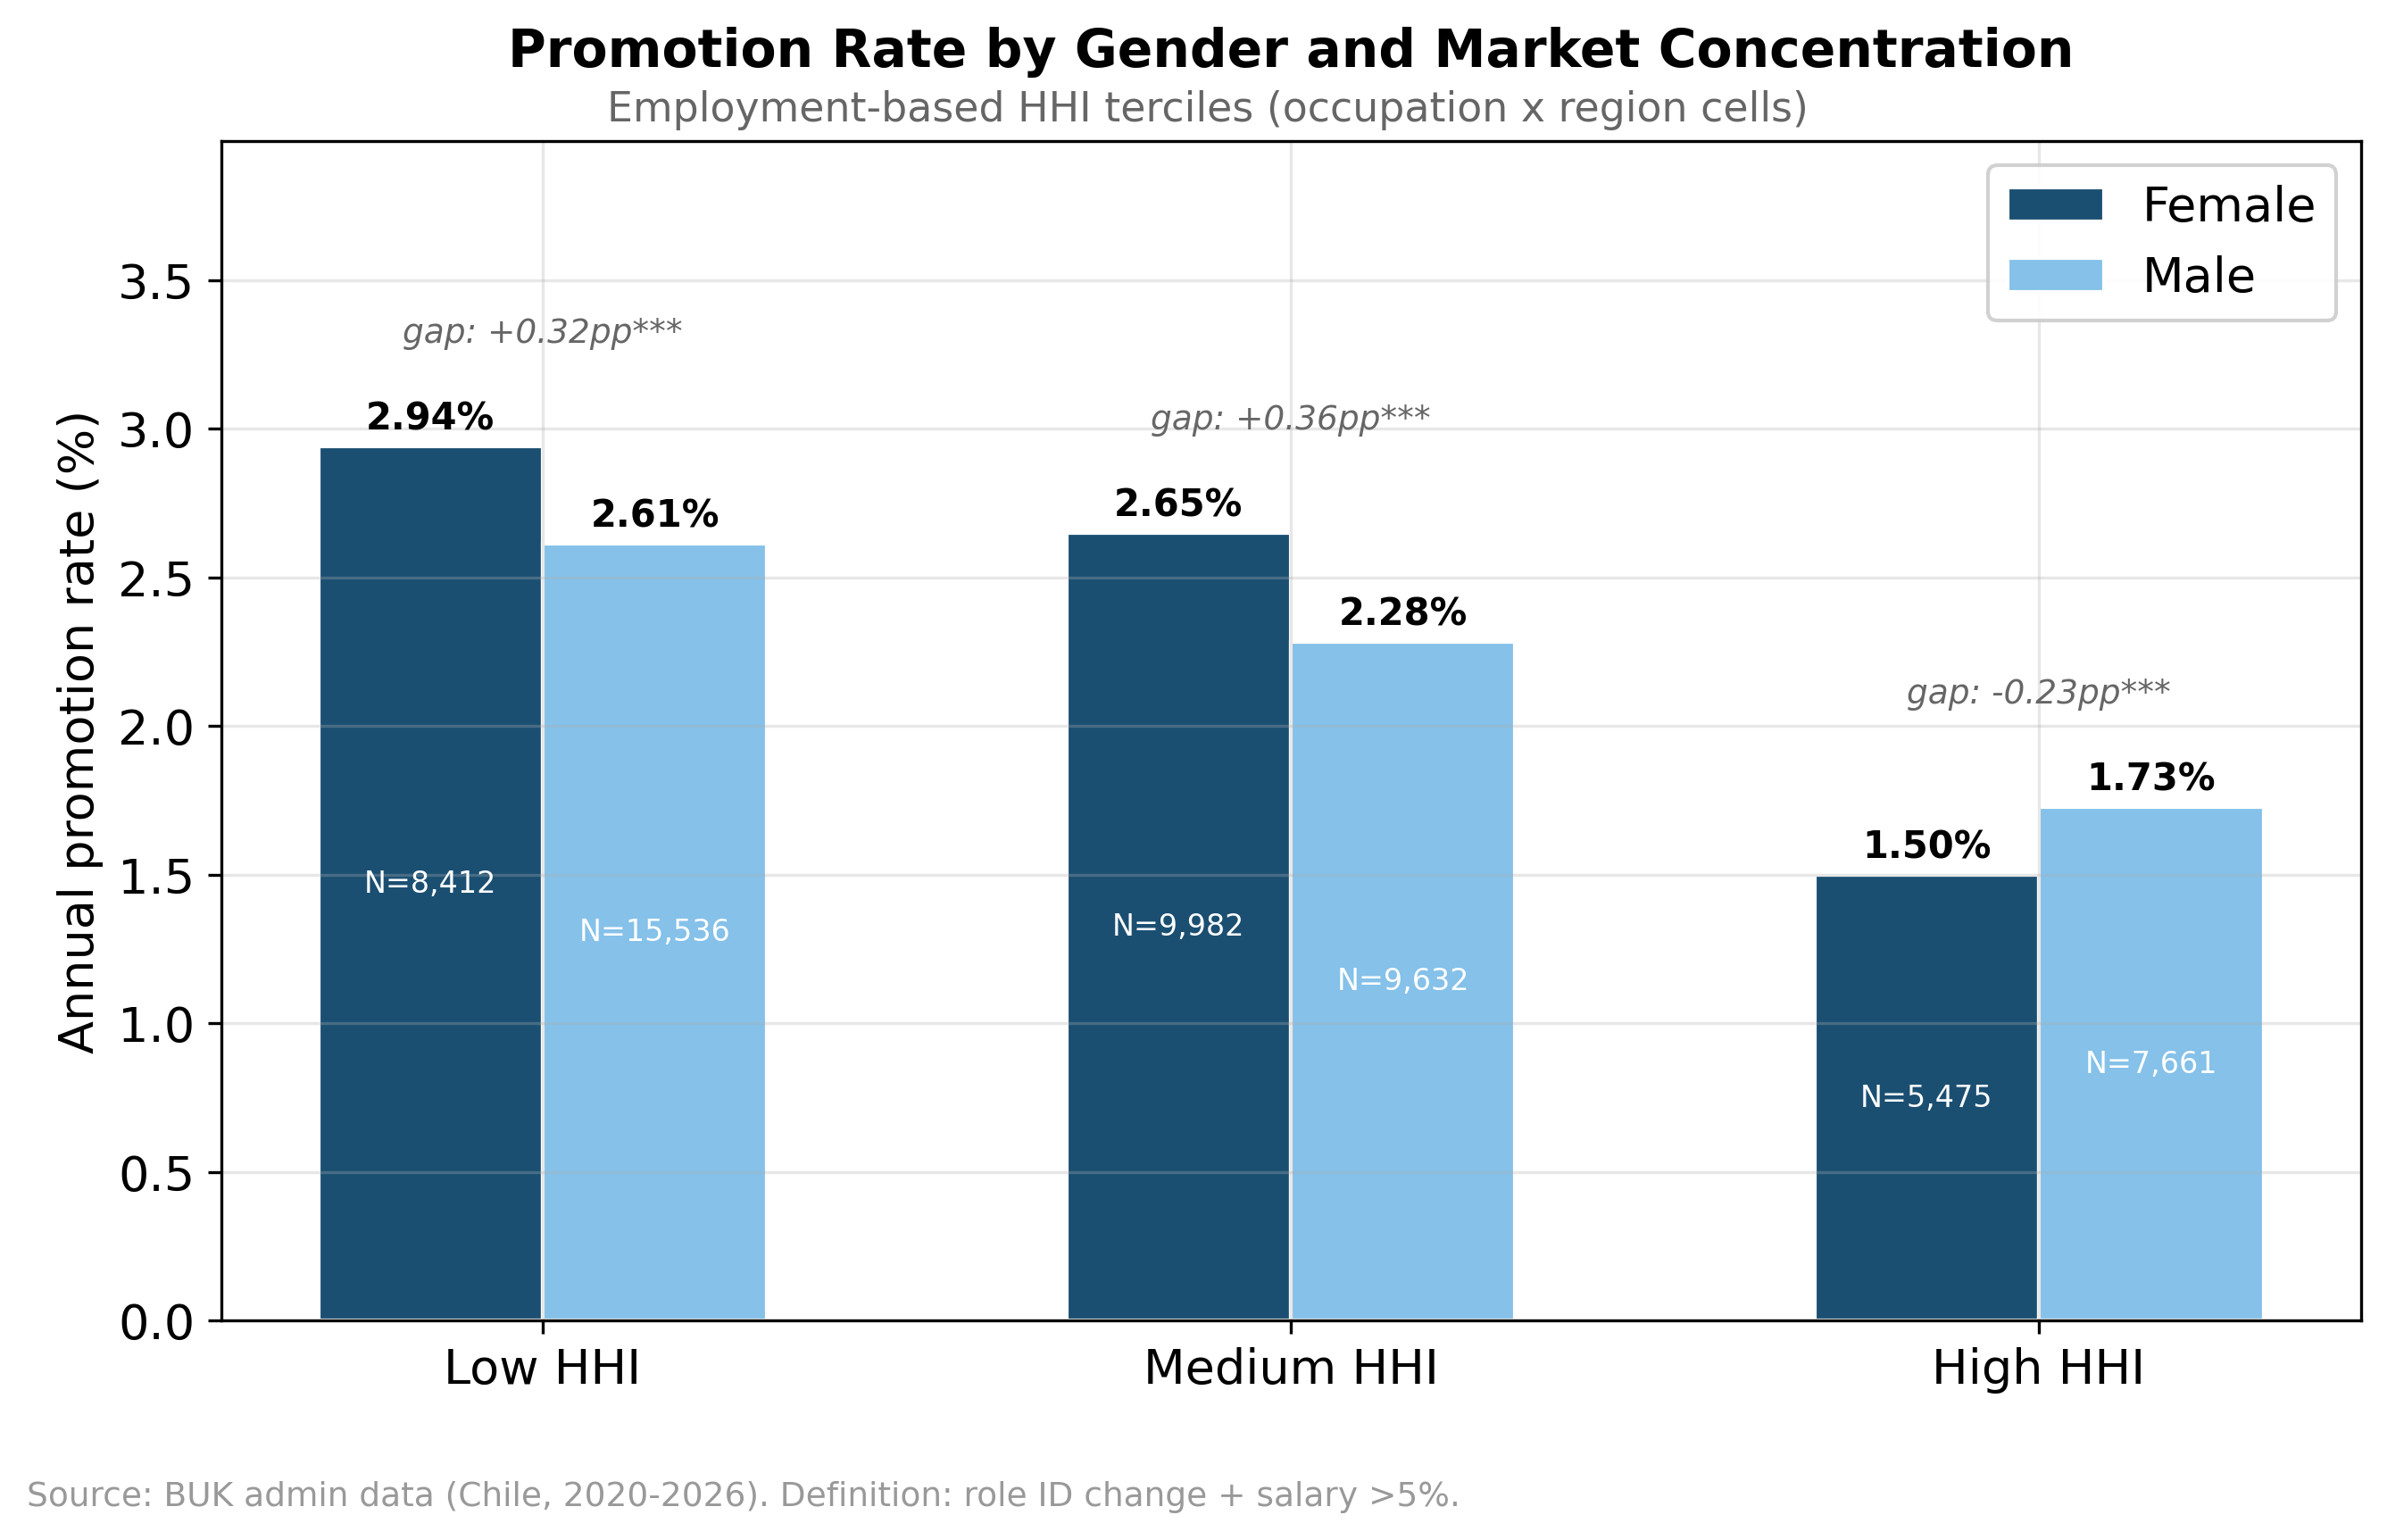
\includegraphics[width=0.72\textwidth]{../../../1_Code/figures/rf_4_3_promotion_by_gender_hhi.png}
\caption{Promotion rate by gender and employment-based HHI tercile (Chile, 2020--2026). Promotion defined as role ID change with salary increase $>$5\%.}
\label{fig:promo_hhi}
\end{figure}

\paragraph{Survey evidence on perceived inequity.} Survey data from the Work in Progress (WiP) 2026 questionnaire support these administrative patterns (see Appendix Figures~\ref{fig:survey_payeq}--\ref{fig:survey_attributes}). Three findings stand out. First, women perceive less pay equity than men, and this perception gap widens with organization size, paralleling the HHI interaction in the promotion data. Second, women report fewer promotion opportunities and face worse outcomes at every stage of the salary negotiation process. Third, lack of growth is the top reason workers of both genders cite for wanting to change jobs, underscoring that career advancement is a first-order concern in this labor market.

\paragraph{Remaining descriptive work.} Several pieces of evidence that would strengthen the case for the model are still in progress. First, job-to-job transition rates by gender would provide the most direct test of whether women face fewer outside options. BUK data is limited for this purpose because most workers are observed at a single employer within the platform; computing transition rates will require supplementary Chilean administrative records (e.g., unemployment insurance data) that I am in the process of accessing. Second, application-to-hire conversion rates by gender and market concentration would test the model's prediction on hiring screening; the hired variable in the recruitment module is still being constructed. Third, wage growth at promotion by gender and HHI would test whether the promotion gap translates into different wage trajectories or whether firms adjust the wage increment to compensate. Finally, the current HHI relies on BUK employment shares within an 8-category occupation taxonomy; future work will implement structural labor supply elasticity estimates following \citet{sharma_monopsony_2023} and commuting-based market definitions following \citet{Schubert_Stansbury_Taska_2024}, which may better capture the relevant margin of labor market power.
% ============================================================
% 5. MODEL
% ============================================================
\section{Model Framework}

%Time is continuous and the economy is in steady state. 
There are two worker types $g \in \{M, F\}$ and a continuum of firms with productivity $p \sim F(p)$. Each firm has two job levels: junior ($j=0$) and senior ($j=1$), with output $y_j(p) = p \cdot a_j$ where $a_1 > a_0$. The production function is gender-neutral, so gender enters entirely through outside options.

Workers receive outside offers at rate $\lambda_g$, with $\lambda_F < \lambda_M$, and separate exogenously at rate $\delta$. When a worker contacts firm $p$, she draws match quality signal  $q \sim H(q)$ and is hired only if $q \geq q_g^*(p)$\footnote{This quality signal can be thought as the signal that CV's, interviews give of actual match quality}, so the probability of passing the screen is $1 - H\bigl(q_g^*(p)\bigr)$. The value of employment at level $j$ in a firm of type $p$ is
\begin{align*}
    rV_{gj}(p) & = w_{gj}(p) + \lambda_g \int \bigl(1 - H(q_g^*(p'))\bigr) \max\bigl\{V_{g0}(p') - V_{gj}(p),\; 0\bigr\} \, dF(p') \\
    & + \delta\bigl[U_g - V_{gj}(p)\bigr] + \mathbbm{1}_{j=0} \cdot \mu_g(p)\bigl[V_{g1}(p) - V_{g0}(p)\bigr],
\end{align*}
where $\mu_g(p)$ is the endogenous promotion rate and the last term captures the option value of promotion. Each firm chooses four instruments per gender: entry wage $w_{g0}$, senior wage $w_{g1}$, a hiring screening threshold $q_g^*$, and a promotion threshold $\theta_g$ (junior workers draw performance $s \sim G(s)$, promoted if $s \geq \theta_g$, yielding promotion rate $\mu_g = 1 - G(\theta_g)$).

\subsection{The promotion mechanism}

The firm's promotion decision balances two forces. The \textit{direct profit effect} is gender-neutral: promoting raises output ($a_1 > a_0$) but also raises the wage. The \textit{retention effect} depends on gender. Promoting a worker raises her continuation value ($V_{g1} > V_{g0}$), making fewer outside offers attractive and reducing the probability she leaves. This benefit is proportional to $\lambda_g$. The difference in retention between promoted and non-promoted workers is
\begin{equation*}
    \lambda_g \bigl[F_g(V_{g1}) - F_g(V_{g0})\bigr].
\end{equation*}
When $\lambda_g$ is small, the retention motive vanishes and the firm promotes only when the direct profit effect is positive. When $\lambda_g$ is large, retention dominates and the firm promotes aggressively to prevent turnover. Since $\lambda_F < \lambda_M$, the retention motive is weaker for women, and the firm optimally sets a higher promotion bar: $\theta_F^* > \theta_M^*$. Women are under-promoted not because they are less capable, but because they are less likely to leave.

\subsection{The hiring mechanism}

Unlike the promotion result, the model does not deliver a clear prediction on hiring. When $\lambda_F < \lambda_M$, two opposing forces shape the firm's screening threshold. First, a \textit{longer tenure force}: women stay longer, so each hire generates surplus over more periods, pushing the firm to lower its threshold. Second, a \textit{less competition force}: women have fewer alternatives and continue to apply even when the bar is high, allowing the firm to be more selective. The net effect is theoretically ambiguous and depends on the relative magnitudes of these forces.

%\subsection{Predictions}

%The model generates three testable predictions:
%\begin{enumerate}
%    \item \textbf{Promotion gap increases with market power.} The gender gap in promotion rates is larger in more concentrated labor markets, where the retention motive for women is weakest.
%    \item \textbf{Hiring screening varies with concentration.} The direction of the gender gap in screening intensity is an empirical question that varies with market structure.
%    \item \textbf{Reinforcing cycle.} Lower outside options lead to fewer promotions, which lead to lower wage growth, which further depress outside offers---monopsony and career stagnation compound over time.
%\end{enumerate}

% ============================================================
% 6. CONCLUSION
% ============================================================
\section{Conclusion}

This paper connects two literatures that have developed largely in parallel: monopsony in labor markets and gender gaps in career dynamics. The preliminary evidence suggests that the gender promotion gap is not uniform but varies systematically with market concentration, consistent with a retention mechanism in which firms with more market power face less pressure to promote women. The next steps are to complete the reduced-form evidence on hiring and outside options, estimate the structural model using the BUK matched employer-employee-applicant data, and exploit Chile's recent labor market reforms for causal identification.

% ============================================================
% REFERENCES
% ============================================================
\newpage
\bibliographystyle{aer}
\bibliography{../bib}

% ============================================================
% APPENDIX
% ============================================================
\newpage
\appendix
\section{Appendix Figures}

\subsection{Survey evidence}

The Work in Progress (WiP) 2026 survey was administered to 6,789 workers currently employed in Chile, Colombia, Mexico, and Peru. The questionnaire covers over 70 questions on compensation, career advancement, work-life balance, and job preferences. The survey is open (not restricted to BUK platform users) and cannot be linked to the administrative records. Figures below restrict the sample to the Chilean subsample.

\begin{figure}[H]
\centering
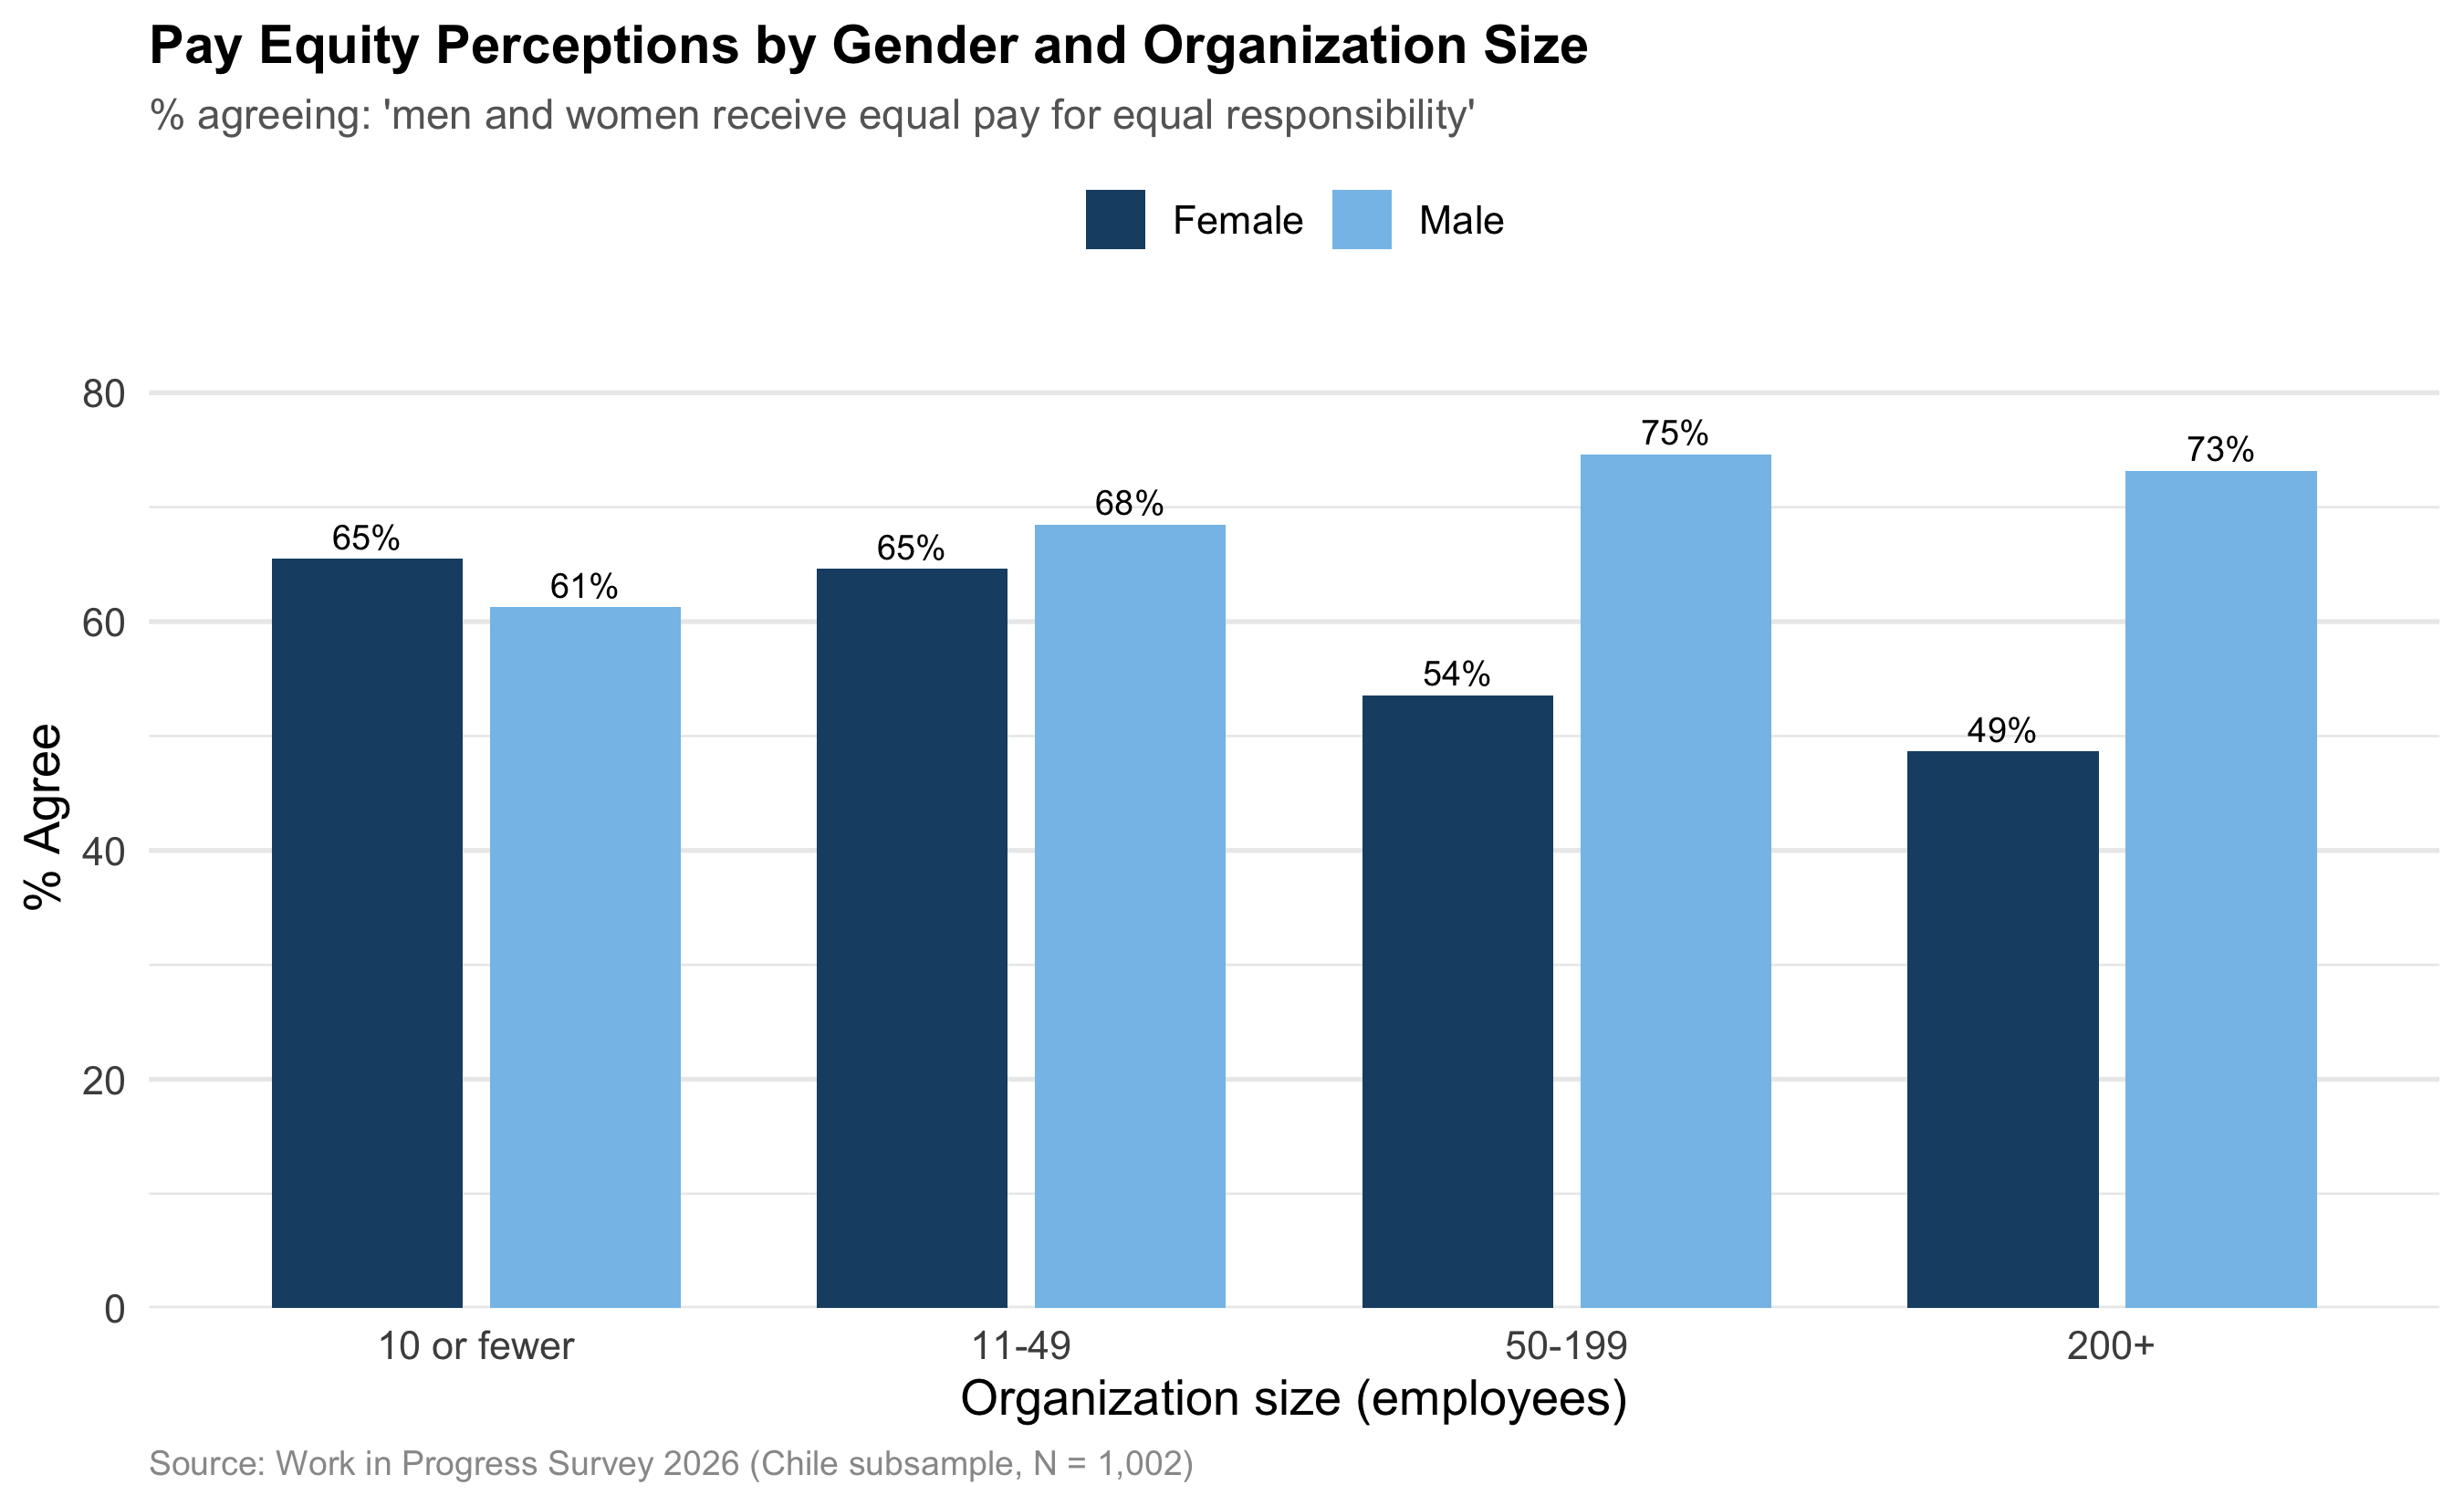
\includegraphics[width=0.72\textwidth]{../../../1_Code/figures/rf_5_6_pay_equity_by_gender_x_orgsize.png}
\caption{Pay equity perceptions by gender and organization size. Share agreeing that ``men and women receive equal pay for equal responsibility.'' Source: WiP Survey 2026, Chile subsample (N = 1,002).}
\label{fig:survey_payeq}
\end{figure}

\begin{figure}[H]
\centering
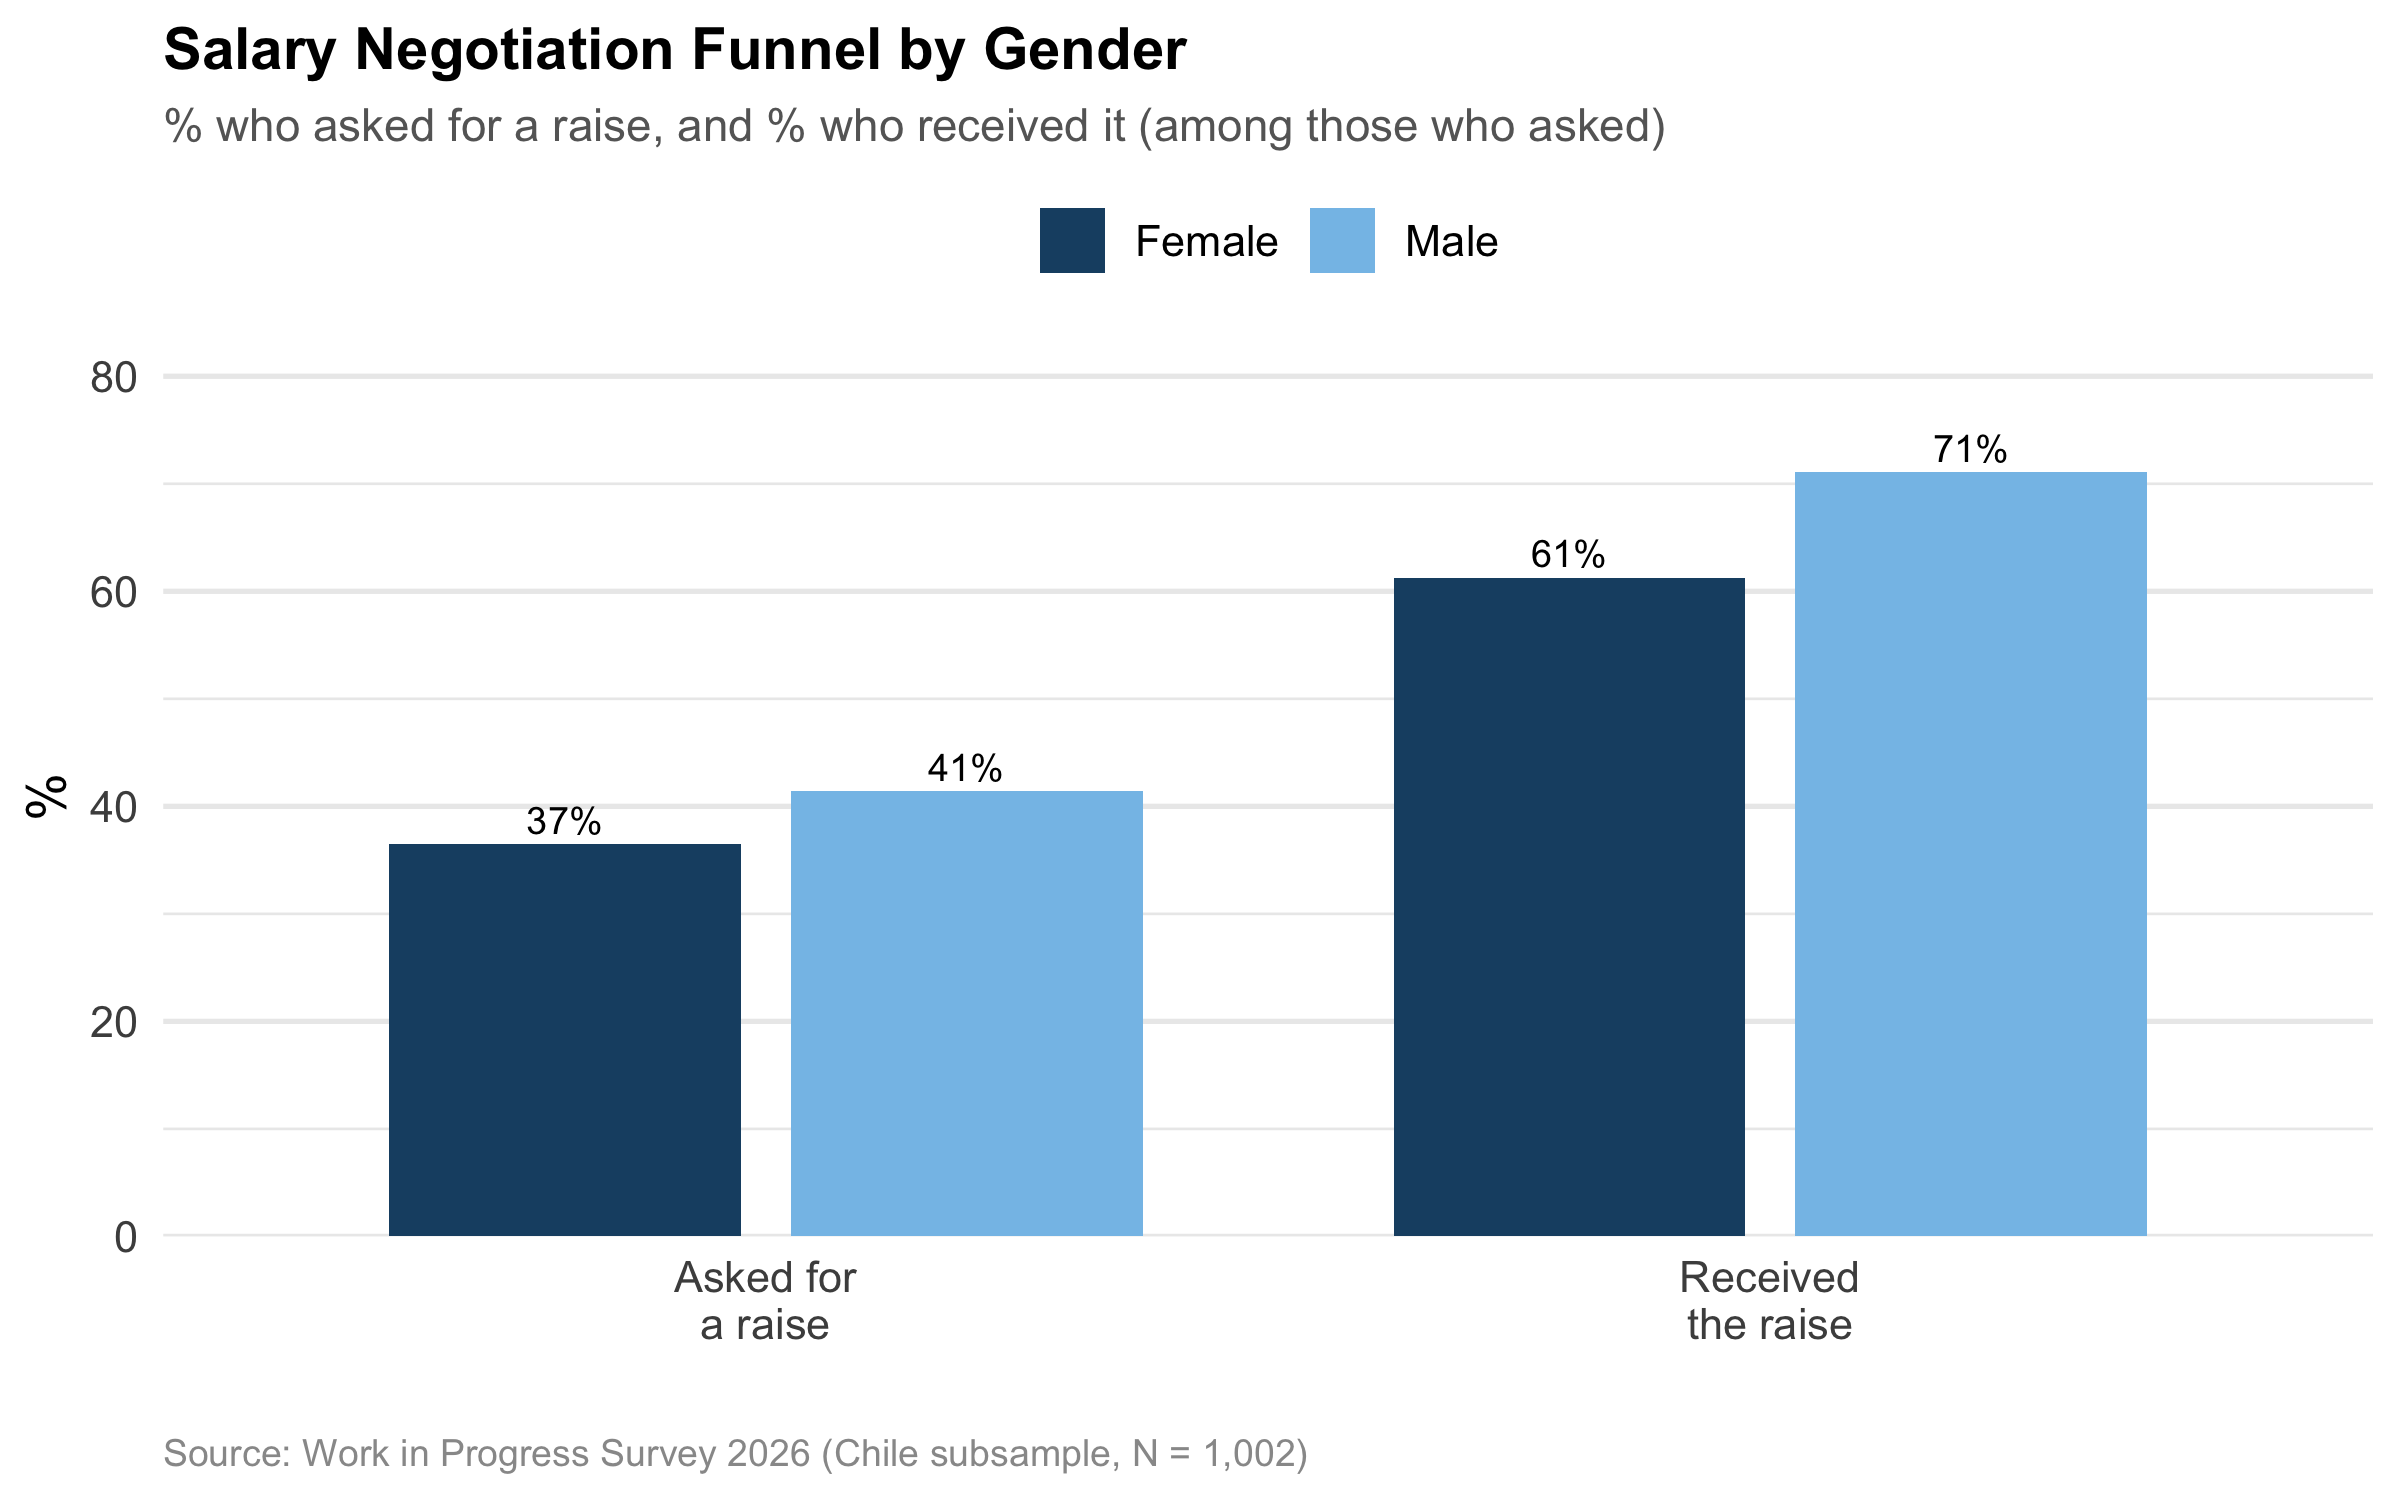
\includegraphics[width=0.72\textwidth]{../../../1_Code/figures/rf_5_2_negotiation_funnel_by_gender.png}
\caption{Salary negotiation funnel by gender: share who asked for a raise and share who received one (conditional on asking). Source: WiP Survey 2026, Chile subsample (N = 1,002).}
\label{fig:survey_negotiation}
\end{figure}

\begin{figure}[H]
\centering
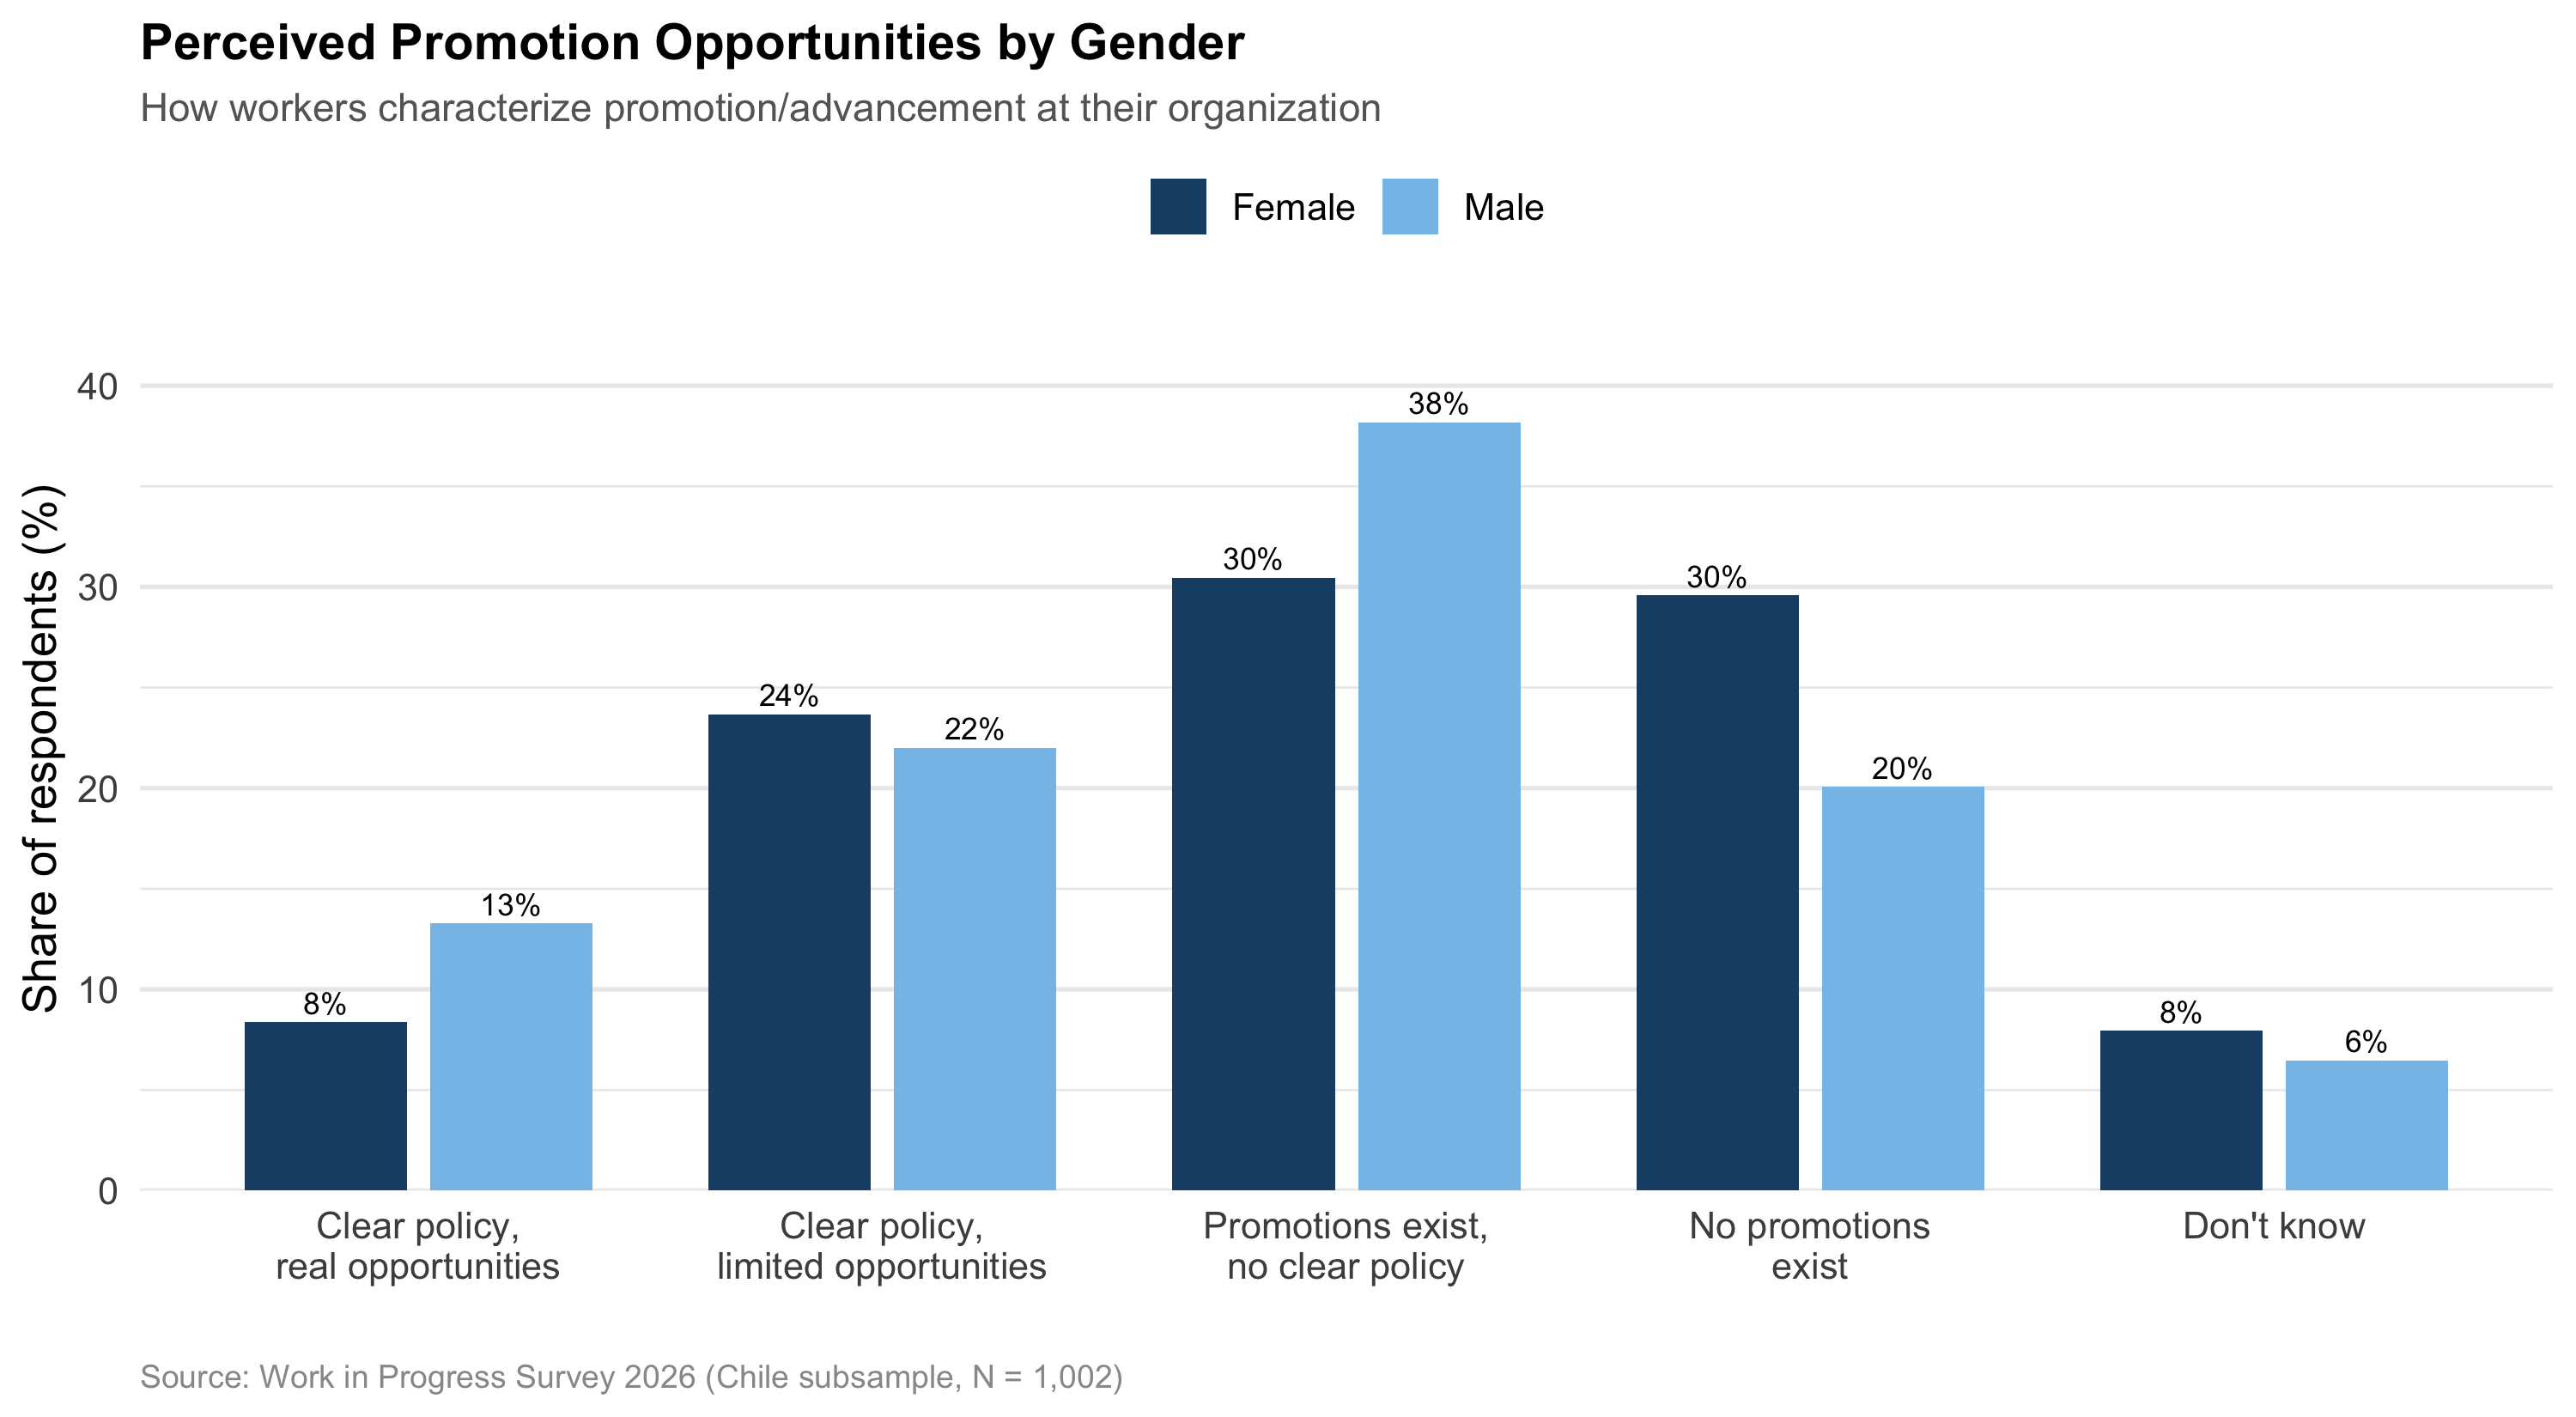
\includegraphics[width=0.72\textwidth]{../../../1_Code/figures/rf_1_7_promotion_perceptions_by_gender.png}
\caption{Perceived promotion opportunities by gender. Workers characterize promotion and advancement possibilities at their organization. Source: WiP Survey 2026, Chile subsample (N = 1,002).}
\label{fig:survey_promoperceptions}
\end{figure}

\begin{figure}[H]
\centering
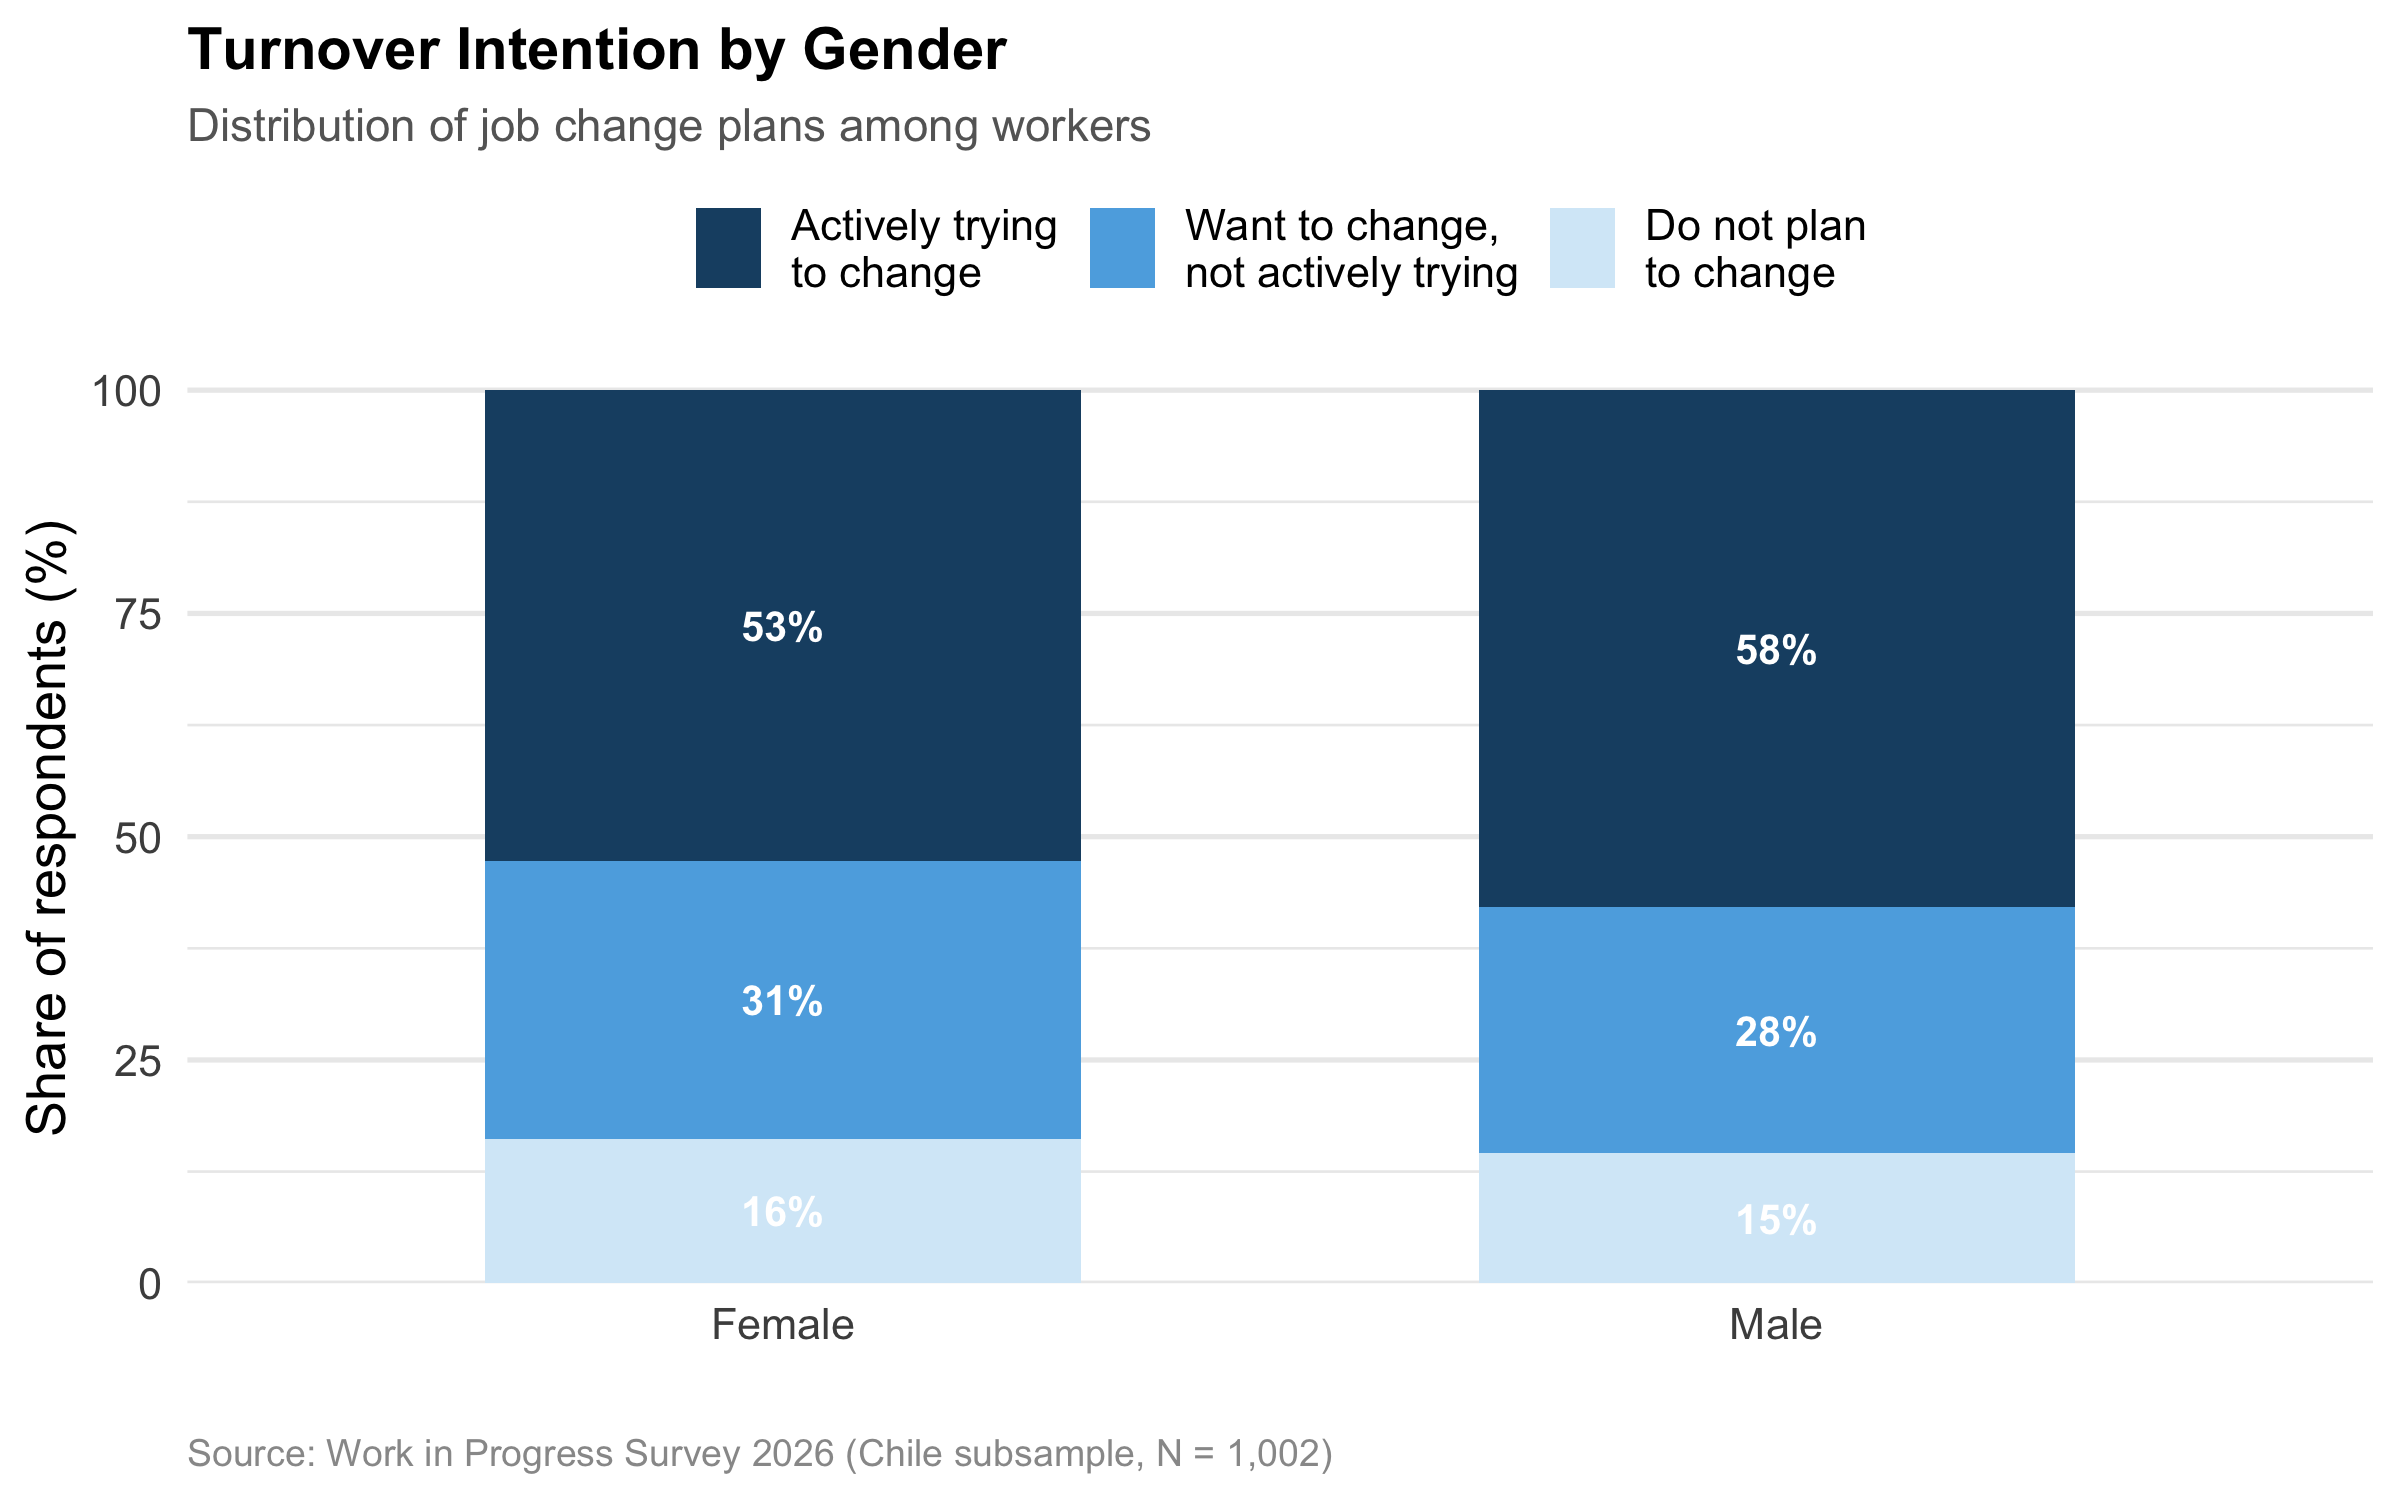
\includegraphics[width=0.72\textwidth]{../../../1_Code/figures/rf_1_5_turnover_intention_by_gender.png}
\caption{Turnover intention by gender: distribution of job change plans among workers. Source: WiP Survey 2026, Chile subsample (N = 1,002).}
\label{fig:survey_turnover}
\end{figure}

\begin{figure}[H]
\centering
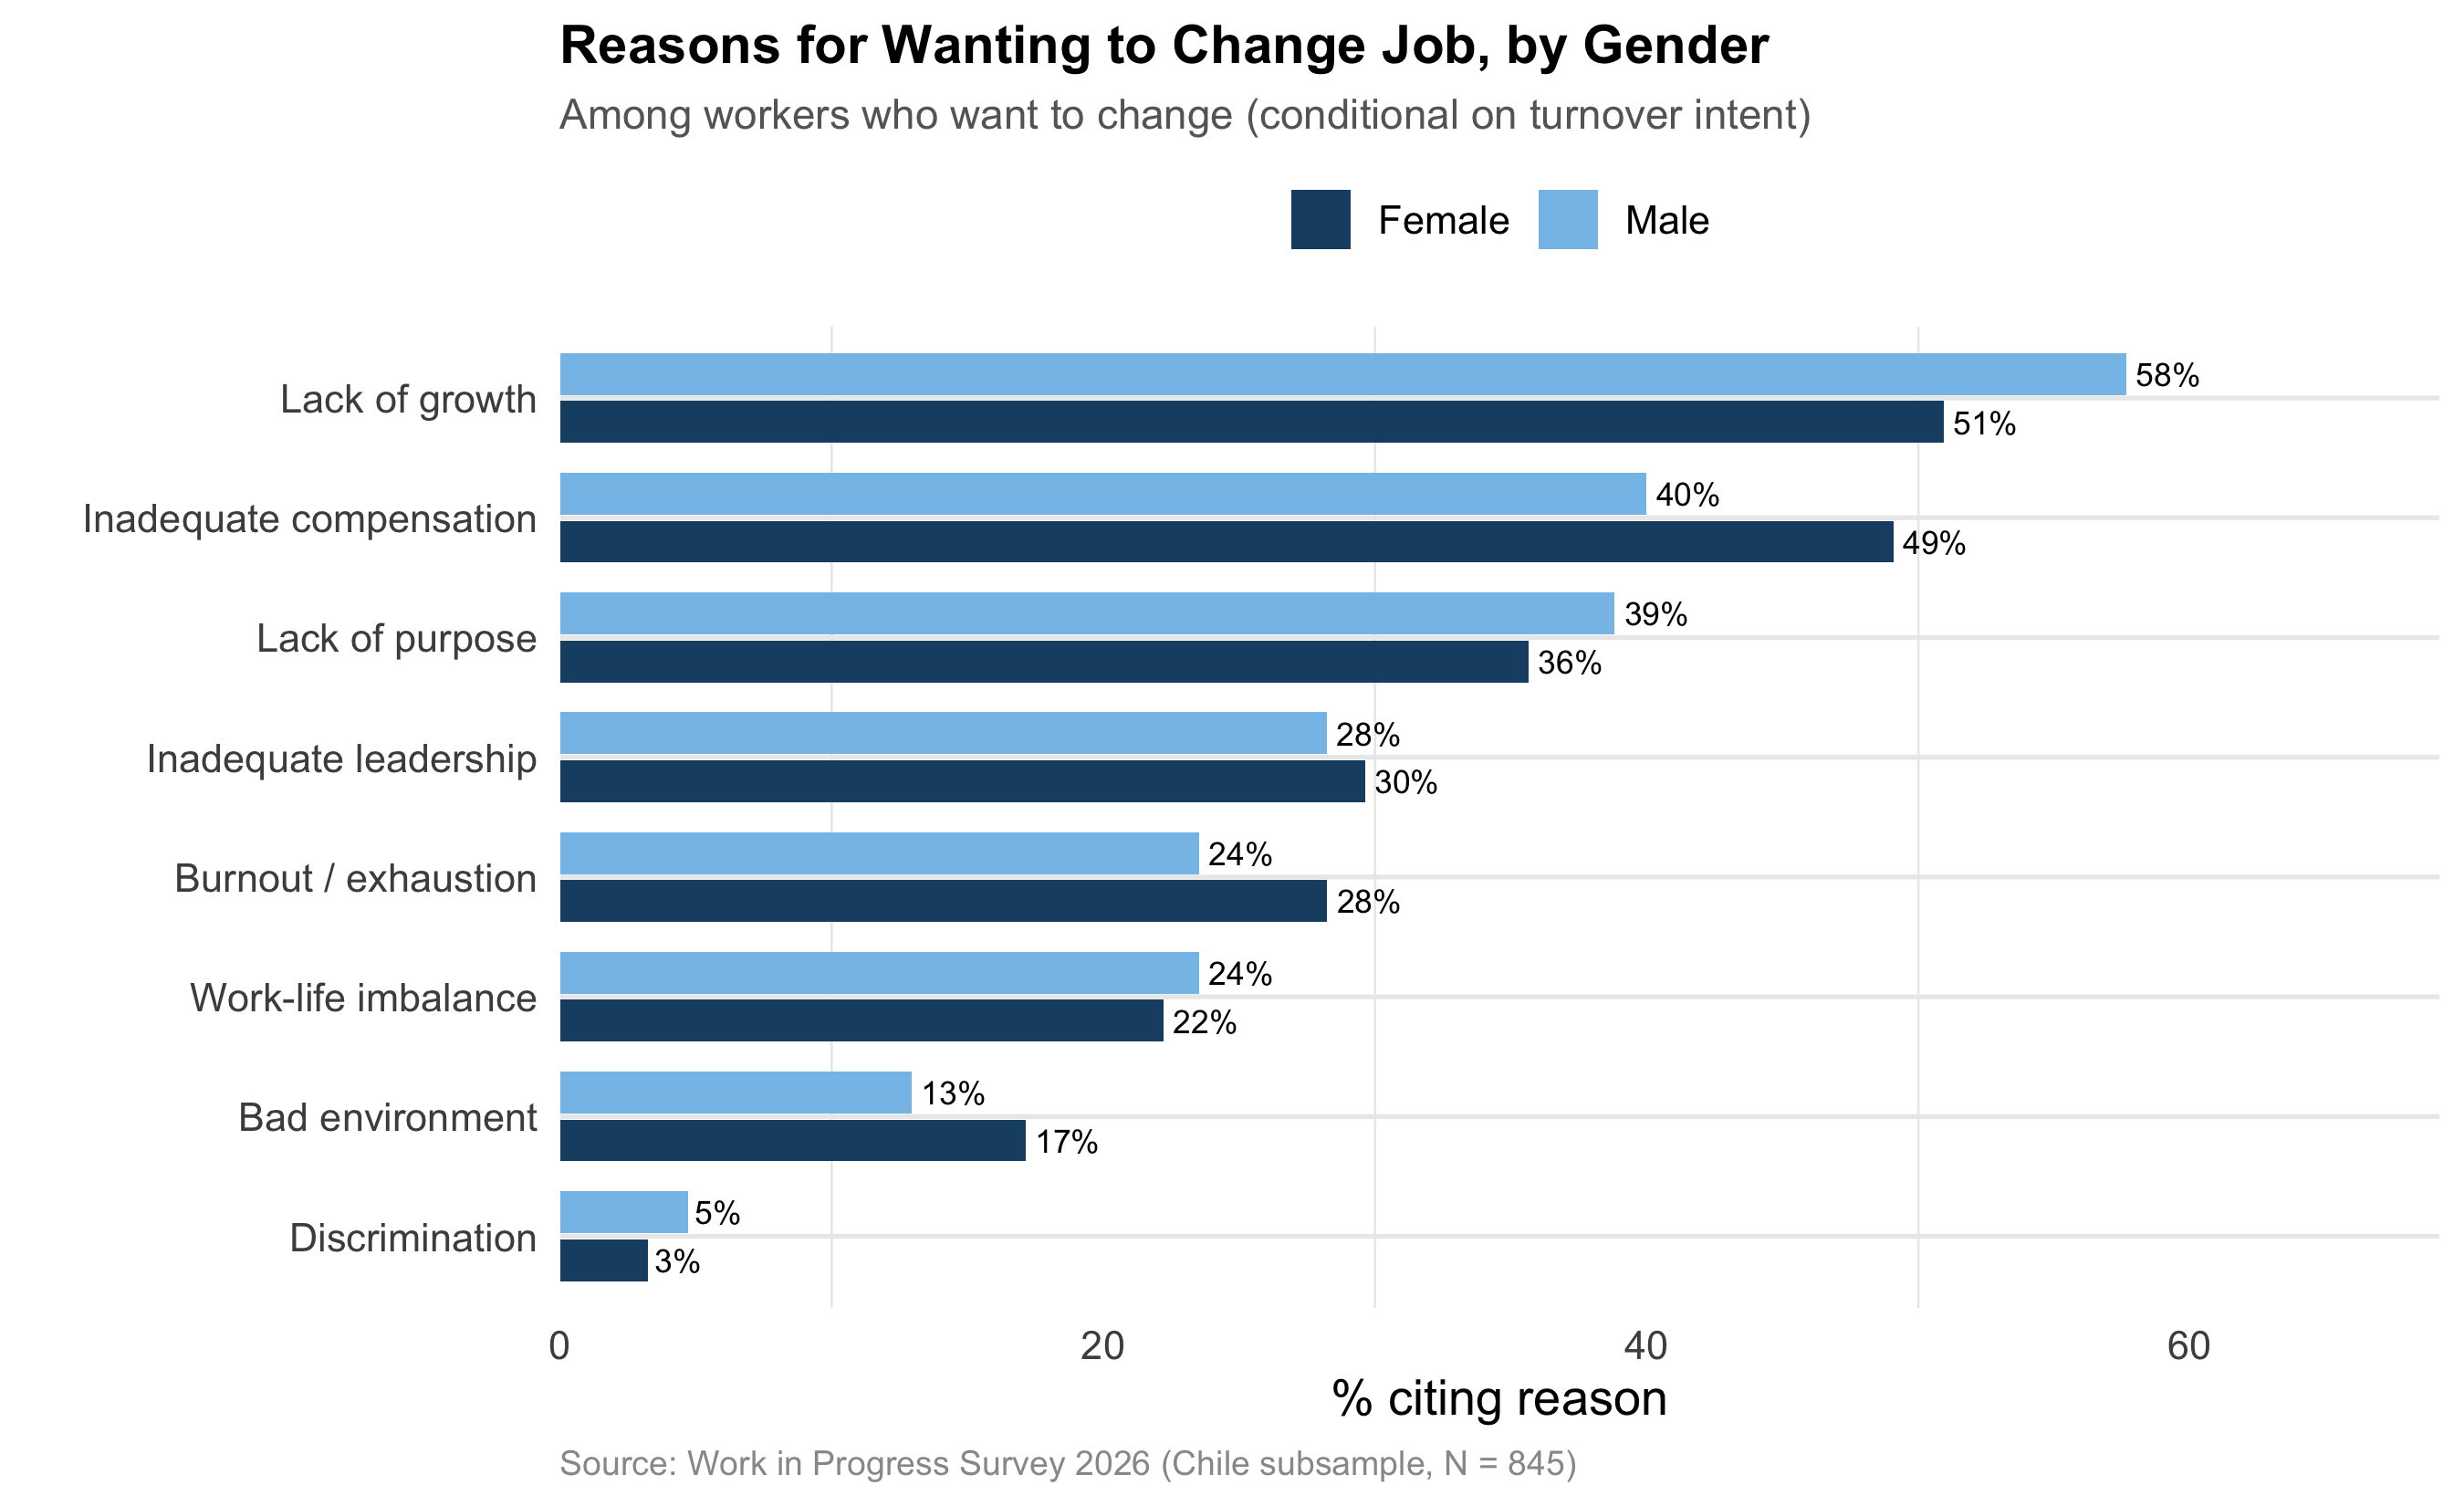
\includegraphics[width=0.72\textwidth]{../../../1_Code/figures/rf_1_6_turnover_reasons_by_gender.png}
\caption{Reasons for wanting to change jobs, by gender (conditional on turnover intent). Source: WiP Survey 2026, Chile subsample (N = 845).}
\label{fig:survey_attributes}
\end{figure}

\subsection{Administrative data}

\begin{figure}[H]
\centering
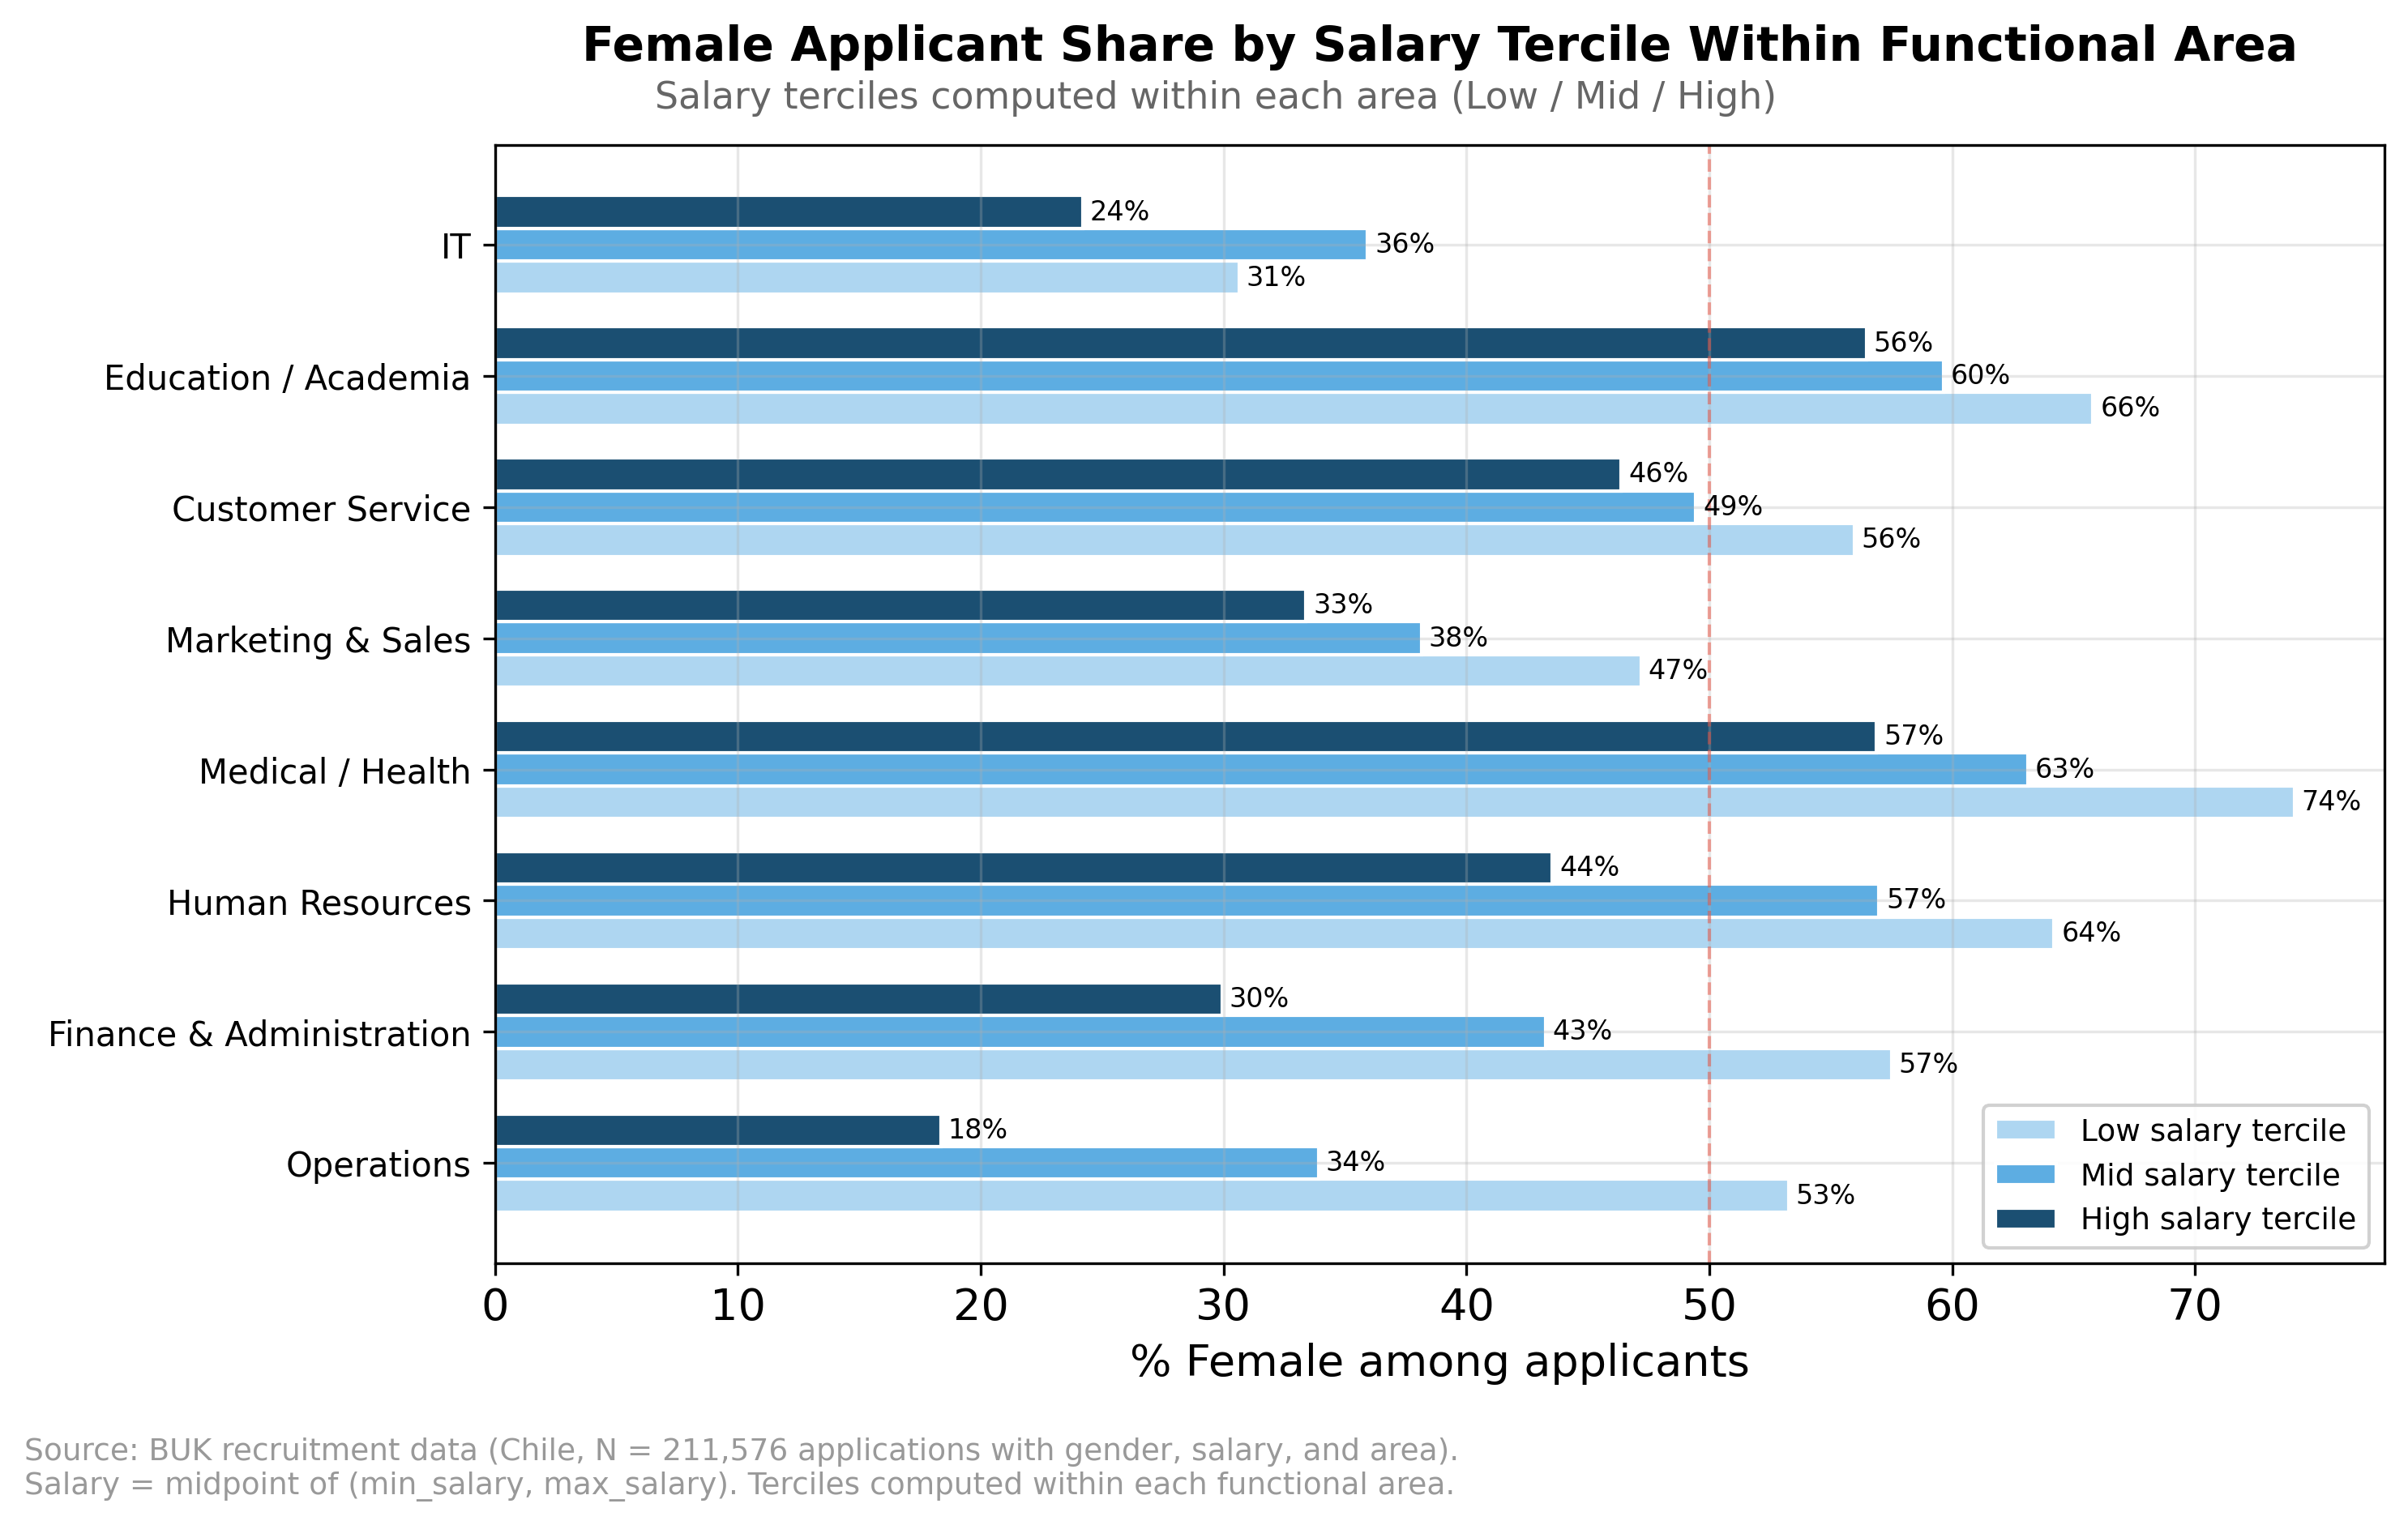
\includegraphics[width=0.72\textwidth]{../../../1_Code/figures/rf_3_5c_female_share_by_salary_within_area.png}
\caption{Female share of applicant pool by posted salary range, within functional area.}
\label{fig:admin_femaleshare}
\end{figure}

\begin{figure}[H]
\centering
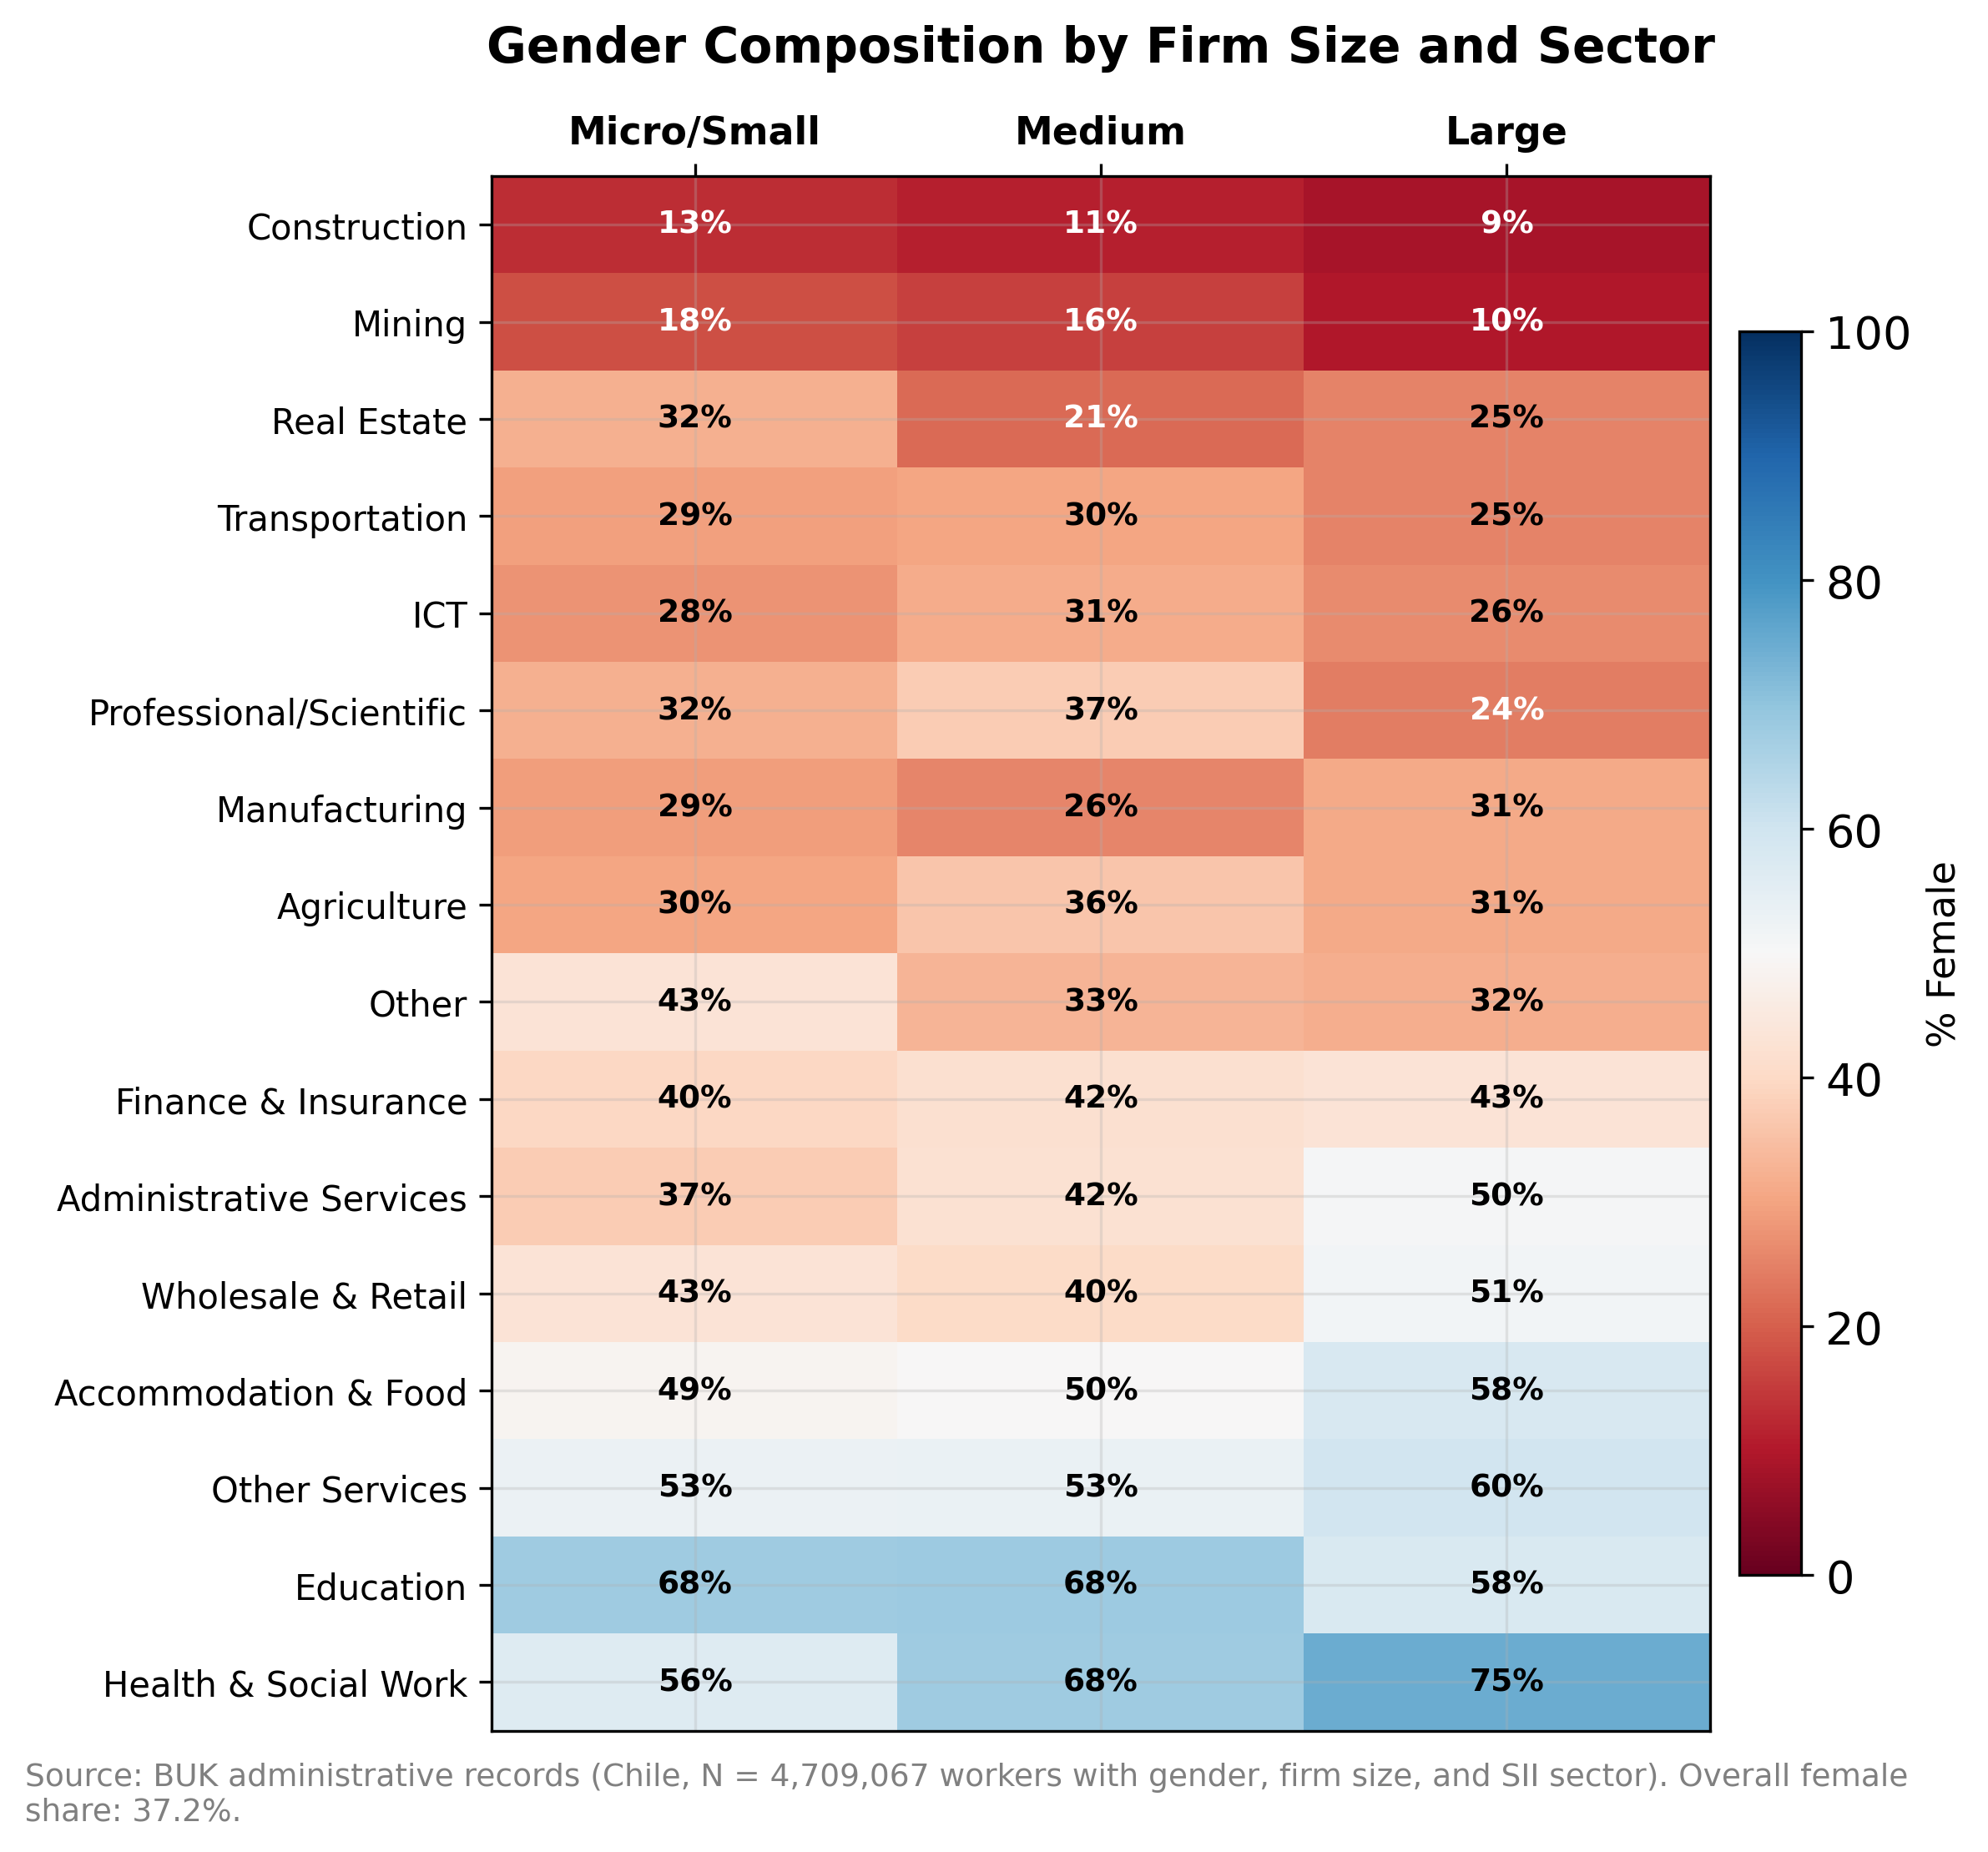
\includegraphics[width=0.72\textwidth]{../../../1_Code/figures/rf_6_3_gender_composition.png}
\caption{Gender composition of BUK firms by sector and firm size.}
\label{fig:admin_gendercomp}
\end{figure}

\begin{figure}[H]
\centering
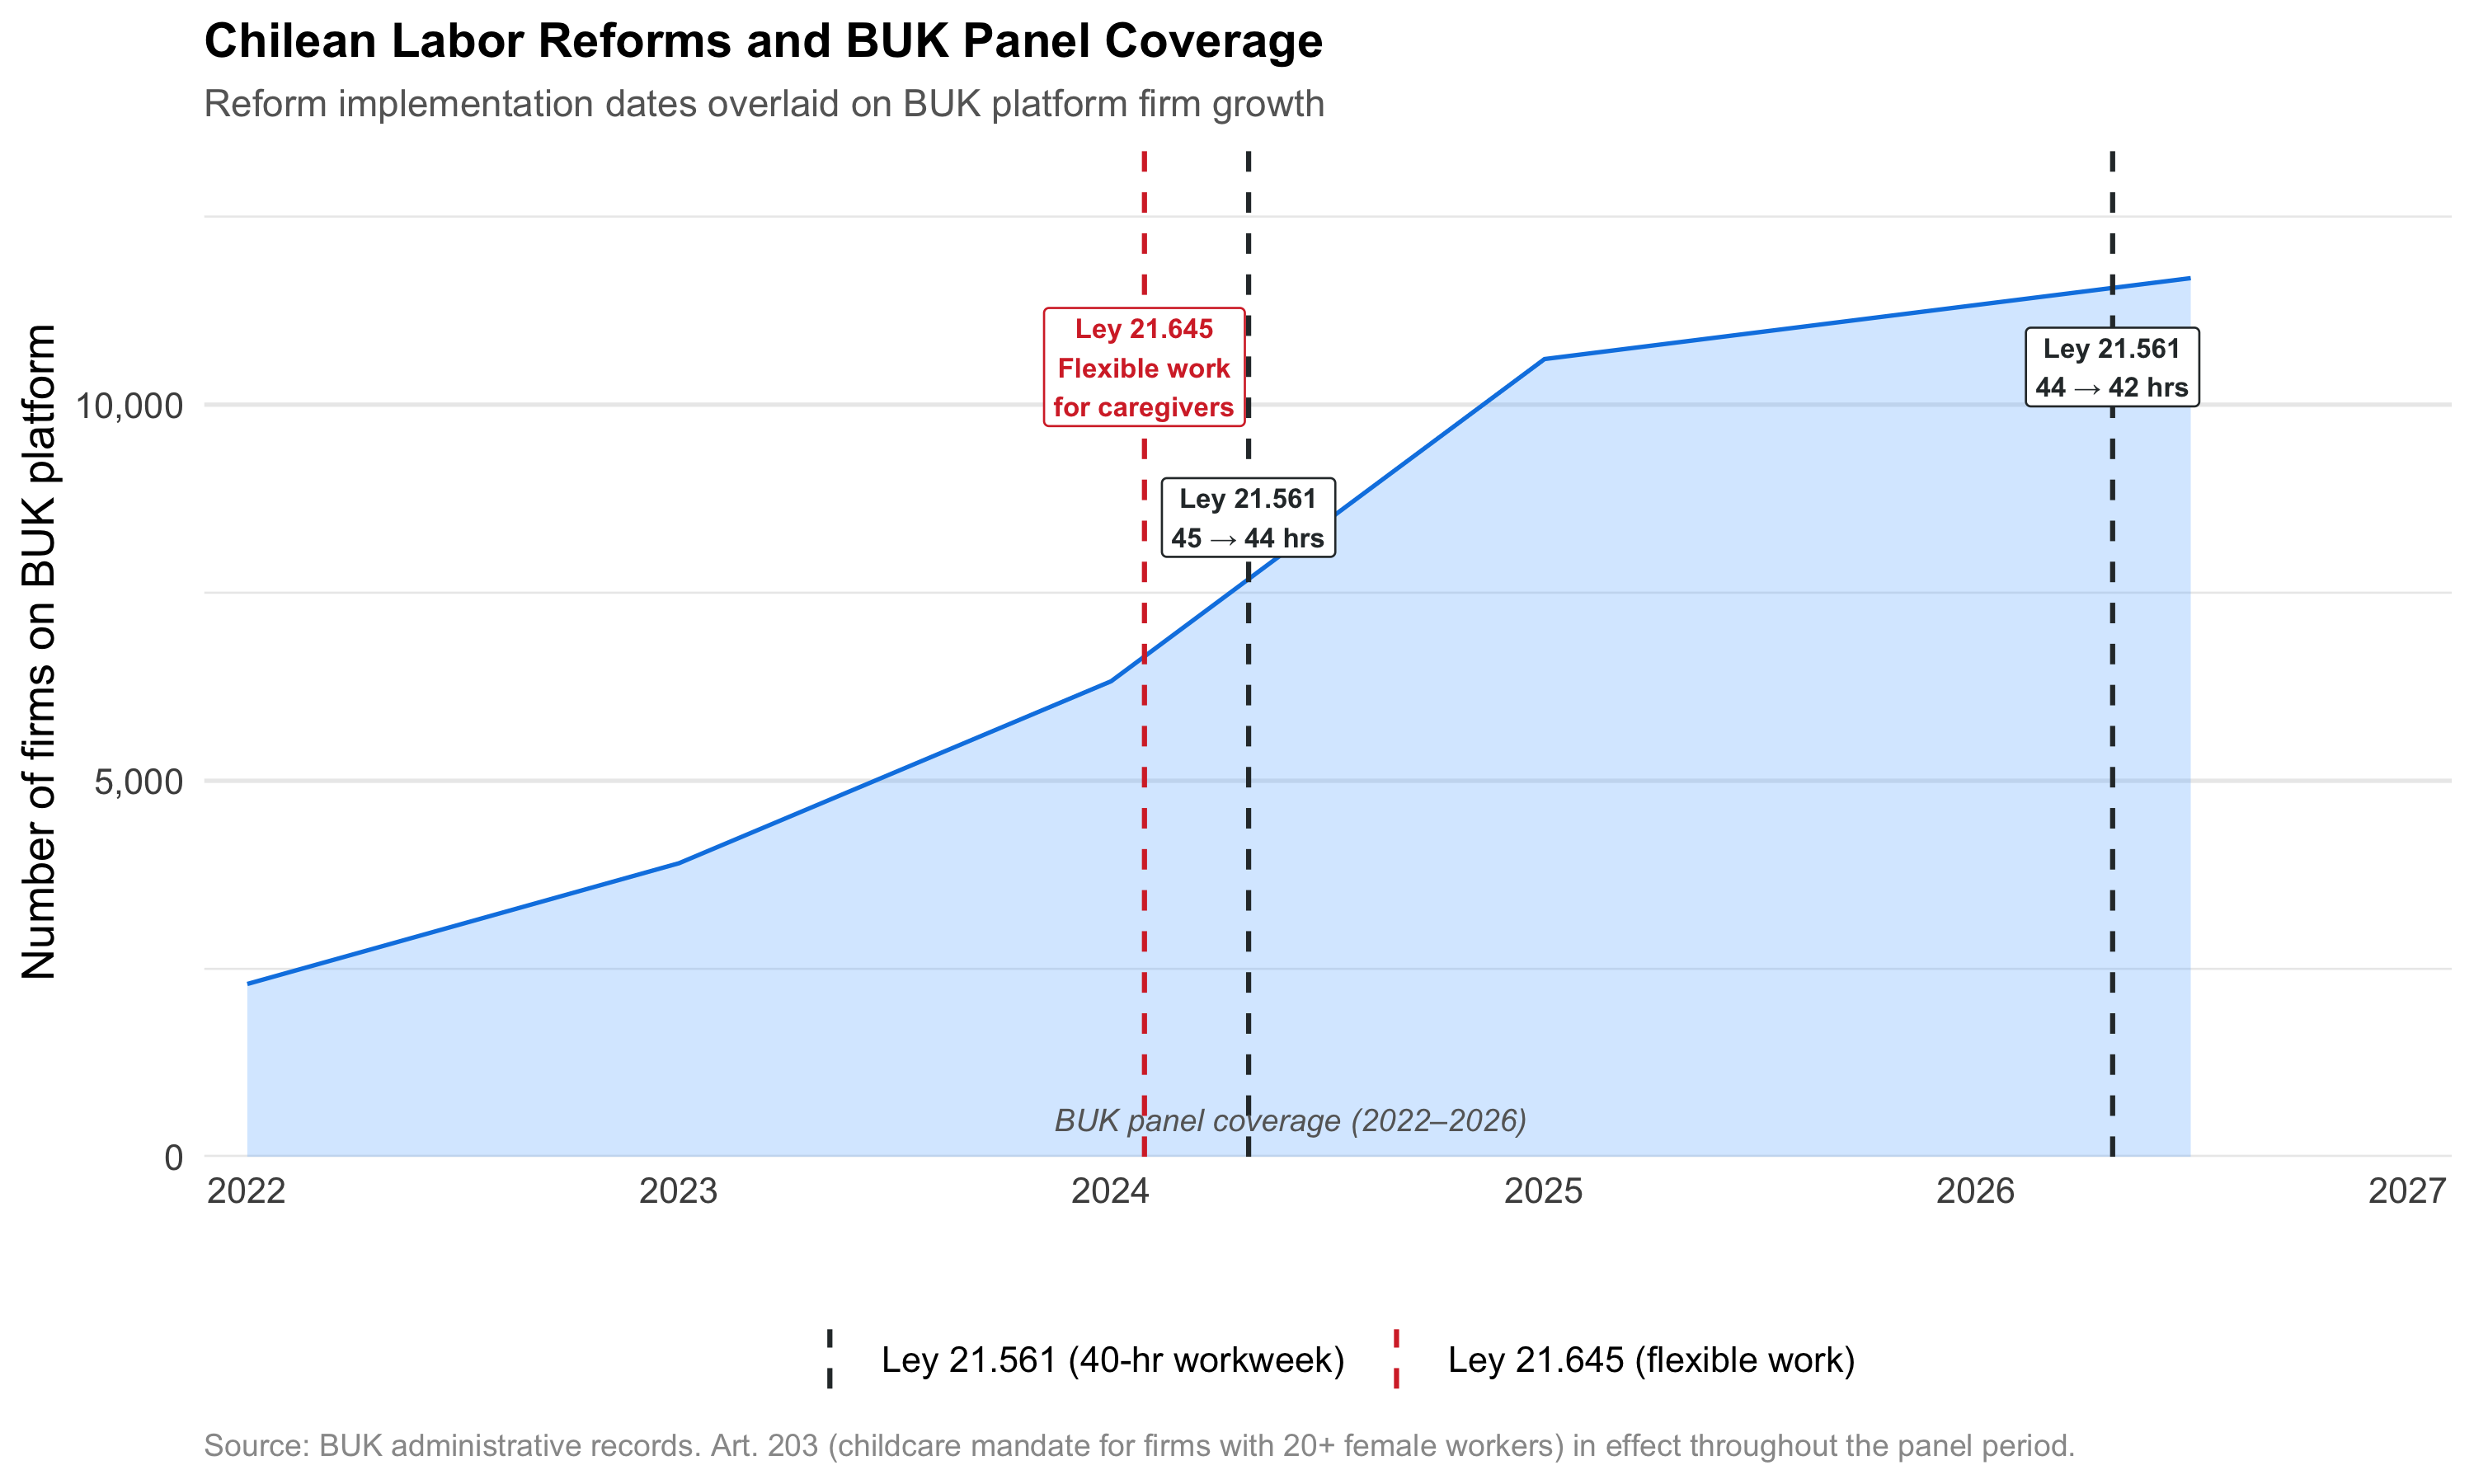
\includegraphics[width=0.72\textwidth]{../../../1_Code/figures/rf_6_4_reform_timeline.png}
\caption{Timeline of Chilean labor market reforms and BUK panel coverage (2022--2026).}
\label{fig:admin_reforms}
\end{figure}

\begin{figure}[H]
\centering
\includegraphics[width=0.72\textwidth]{../../../../4_Code/images/heatmap_coverage.png}
\caption{BUK coverage rate (BUK firms / SII firms) by ISIC sector and firm size, pooled 2020--2023.}
\label{fig:admin_coverage}
\end{figure}

\end{document}
